\newif\ifdraft %XXX
\drafttrue % \draftfalse %XXX

%%%--- Template for master thesis at SfS
%%%--- Modified template with more comments and examples -- SG, 11/06/09
%%%------
\ifdraft \documentclass[11pt,a4paper]{report} \else%XXX
\documentclass[11pt,a4paper,twoside,openright]{report}
\fi %XXX
\usepackage[english]{sty/ETHDAsfs}%--> ETHDASA + fancyhdr + ... "umlaute"
%  + sfs-hyper -> hyperref 

\usepackage{pdfpages}%%to include the confirmation of originality (plagiarism
\usepackage{amsbsy}%% for \boldsymbol and \pmb{.}
\usepackage{amssymb}%% calls  amsfonts...
\usepackage{graphicx}%-- für PostScript-Grafiken (besser als  psfig!)
%\usepackage[draft]{graphicx} % grafics shown as boxes --> faster compilation
%
\usepackage[longnamesfirst]{natbib}%was {sfsbib}%- Für  Literatur-Referenzen
%           ^^^^^^^^^^^^^^ 1) "Hampel, Ronchetti, ..,"  2) "Hampel et al"
% Engineers (and other funny people) want to see [1], [2] 
% ---> use 'numbers' : \usepackage[longnamesfirst,number]{natbib}
%
%
\usepackage{sty/texab}%- 'tex Abkürzungen' /u/sfs/tex/tex/latex/texab.sty
        %%- z.B.  \R, \Z, \Q, \Nat für reelle, ganze, rationale, natürl. Zahlen;
        %%-       \N   (Normalvert.)  \W == Wahrscheinlichkeit .....
        %%-  \med, \var, \Cov, \....
        %%-  \abs{x} == |x|   und   \norm{y} ==  || y ||   (aber anständig)
%% NOTE: texab contains many useful definitions and "shortcuts". It is
%% worth to open the file and have a look at them. HOWEVER, some
%% definitions are a bit can lead to conflicts with other packages. You
%% might for example want to comment out the line defininf \IF as an
%% operator when working with the algorithmic package, or to comment out
%% the line defining a command \Cite with working with the Biblatex package  
\usepackage{amsmath}
%\usepackage{mathrsfs}% Raph Smith's Formal Script font --> provides \mathscr
\usepackage[utf8]{inputenc}% <<------- Unicode, *NOT* iso-latin1 !
\usepackage{ae}% A[lmost] E[uropean] Fonts
\usepackage{enumerate}% Fuer selbstdefinierte Nummerierungen
%--------
\usepackage{relsize}%-> \smaller (etc) used here
\usepackage{color} %% to allow coloring in code listings
\usepackage{pgf}
% for my table env
  \usepackage{booktabs}
  \usepackage{tabularx}
  \usepackage{lipsum}
  \usepackage{enumitem} %for compact itemize
  % \usepackage{paralist} % cpk itemeze
  \usepackage{makecell} %for table 
%-------
\usepackage{listings}% Fuer R-code, C-code, ....  and settings for these:
% listings
  \definecolor{Mygrey}{gray}{0.75}% for linenumbers and only!
  \definecolor{Cgrey}{gray}{0.4}% for comments
  \lstloadlanguages{R}
  %%--- first version of "listings of R"-style : ---------------------------
  % %% using \smaller here: makes R code listings use a *small* font:
  % \lstset{language=R,basicstyle=\smaller[2],commentstyle=\rmfamily\smaller,
  %   showstringspaces=false,xleftmargin=4ex,
  %   literate={<-}{{$\leftarrow$}}1 {~}{{$\sim$}}1}
  % \lstset{escapeinside={(*}{*)}} % for (*\ref{ }*) inside lstlistings (Scode) 
  %\newcommand{\lil}[1]{\lstinline|#1|}
  %%--- newer version of "listings of R"-style : ---------------------------
  \lstset{%% Help, e.g. --> https://en.wikibooks.org/wiki/LaTeX/Source_Code_Listings
    language=R,
    basicstyle=\ttfamily\scriptsize,%%- \small > \footnotesize > \scriptsize > \tiny
    %commentstyle=\ttfamily\color{Cgrey},
    commentstyle=\itshape\color{Cgrey},
    numbers=left,
    numberstyle=\ttfamily\color{Mygrey}\tiny,
    stepnumber=1,
    numbersep=5pt,
    backgroundcolor=\color{white},
    showspaces=false,
    showstringspaces=false,
    showtabs=false,
    frame=single,
    tabsize=2,
    captionpos=b,
    breaklines=true,
    %breakatwhitespace=false,
    keywordstyle={},
    morekeywords={},
    xleftmargin=4ex, 
    literate={<-}{{$\leftarrow$}}1 {~}{{$\sim$}}1
  }
  \lstset{escapeinside={(*}{*)}} % for (*\ref{ }*) inside lstlistings (Scode) 
%%----------------------------------------------------------------------------

%%------- Theoreme ---
\newtheorem{definition}{Definition}[subsection]
\newtheorem{lemma}[definition]{Lemma}
\newtheorem{theorem}[definition]{Theorem}
\newtheorem{Coro}[definition]{Corollary}
\theoremstyle{definition} 
\newtheorem{example}[definition]{Example}
\newtheorem*{note}{Note}
\newtheorem*{remark}{Remark}

\DeclareMathOperator*{\plim}{plim}
% \def\MR#1{\href{http://www.ams.org/mathscinet-getitem?mr=#1}{MR#1}}

% \newcommand{\Lecture}[3]{\marginpar{#3.#2.#1}}
% \newcommand{\Fu}{\mathcal{F}}
\newcommand{\aatop}[2]{\genfrac{}{}{0pt}{}{#1}{#2}}

%\renewcommand{\theequation}{\arabic{equation}}
\numberwithin{equation}{subsection}

%%%%%%%%%%%%%%%%%%%%%%%%%%%%%%%%%%%%%%%%%%%%%%%%%
%%% Path for your figures                      %%%
%%%%%%%%%%%%%%%%%%%%%%%%%%%%%%%%%%%%%%%%%%%%%%%%%
% Set the paths where all figures are taken from:
\graphicspath{{./figures/}}

%%%%%%%%%%%%%%%%%%%%%%%%%%%%%%%%%%%%%%%%%%%%%%%%%
%%% Define your own commands here             %%%
%%%%%%%%%%%%%%%%%%%%%%%%%%%%%%%%%%%%%%%%%%%%%%%%%
\newcommand{\Bruch}[2]{{}^{#1}\!\!/\!_{#2}}
\renewcommand{\labelenumi}{\roman{enumi}.)}
\ifdraft \usepackage{lineno} \linenumbers  %XXX
\definecolor{mygray}{gray}{0.75}
\renewcommand{\linenumberfont}{\normalfont\scriptsize\color{mygray}}
\fi %XXX

\newenvironment{my_figure}[3][t]{
  \begin{figure}[#1]
    \begin{center}
      % \fbox % trim= left bottom right top  % trim= 0.8cm 0.8cm 0.6cm 0.8cm
      \ifdraft \fcolorbox{mygray}{white} {\includegraphics[#2]{#3}} \else
      \includegraphics[#2]{#3} \fi
      % for more options: https://latexref.xyz/_005cincludegraphics.html 
      \label{fig:#3}
}{
    \end{center}
  \end{figure}
}

% Environment for pros and cons table
\newenvironment{my_pros_cons_table}[3][topsep=0pt,parsep=2pt,partopsep=0pt, leftmargin=5pt, rightmargin=-10pt]{
  \begin{table}[h]
    \vspace{-8pt} % remove space before table
    \begin{tabularx}{\linewidth}{>{\parskip1ex}X@{\kern4\tabcolsep}>{\parskip1ex}X}
      % \toprule %makes a bar at the top
      \hfil\bfseries Pros & \hfil\bfseries Cons
      \\\cmidrule(r{3\tabcolsep}){1-1}\cmidrule(l{-\tabcolsep}){2-2}
      \vspace{-11pt} % no gap wetween pros/cons and list
      \begin{itemize}[#1]
        #2
      \end{itemize}
      % \vspace{-11pt} % no effect
      \nointerlineskip & 
      \vspace{-11pt} % no gap wetween pros/cons and list
      \begin{itemize}[#1]
        #3
      \end{itemize}
      % \vspace{-11pt} % no effect
      \nointerlineskip
     \\\bottomrule
    \end{tabularx}
    \vspace{-5pt}
}{\end{table}}


\begin{document}
\bibliographystyle{chicago}% ---> Hampel,F., E.Ronchetti,... W.Stahel(1986) ...
%was \bibliographystyle{sfsbib}\citationstyle{dcu} %OR DEFAULT : \citationstyle{agsm}

\pagenumbering{roman}%- roman numbering for first few pages

%%%%%%%%%%%%%%%%%%%%%%%%%%%%%%%%%%%%%%%%%%%%%%%%%
%%% Title page                                %%%
%%%%%%%%%%%%%%%%%%%%%%%%%%%%%%%%%%%%%%%%%%%%%%%%%
\period{Spring 2022}
\dasatype{Master Thesis}
\students{Lukas Graz}
\mainreaderprefix{Adviser:}
\mainreader{Prof.\ Dr.\ Nicolai Meinshausen}
\alternatereaderprefix{Co-Adviser:}
\alternatereader{Gregor Perich}
\submissiondate{September 18th 2022}
\title{The title of my thesis \\ which should be split on \\ several lines
  if it is too long}

\ifdraft \else%XXX
  \maketitle%- Titelseite wird abgeschlossen
  \cleardoublepage
\fi %XXX
%%~~~~~~~~~~~~~~~~~~~~~~~~~~~~~~~~~~~~~~~~

%%%%%%%%%%%%%%%%%%%%%%%%%%%%%%%%%%%%%%%%%%%%%%%%%
%%% Insert here acknowledgements and abstract %%%
%%%%%%%%%%%%%%%%%%%%%%%%%%%%%%%%%%%%%%%%%%%%%%%%%
%% Dedication (optional)
\ifdraft \else%XXX

  \markright{}
  \vspace*{\stretch{1}}
  \begin{center}
    To some special person
  \end{center}
  \vspace*{\stretch{2}}

  % Preface (optional)
  \newpage
  \markboth{Preface}{Preface}
  \chapter*{Preface}

First words and acknowledgements.

XXX

Betreuung von Gregor

Ideen mit Meinshausen

Resourccen vom SFS

%%% Local Variables: 
%%% mode: latex
%%% TeX-master: "MasterThesisSfS"
%%% End: 


  % Abstract should not be longer than one page.
  \newpage
  \markboth{Abstract}{Abstract}
  \chapter*{Abstract}

%% Intro
Multispectral satellite imagery is used to model vegetation characteristics and development on a large scale in agriculture. As an example, satellite-derived Time Series (TS) of spectral indices like the Normalized Difference Vegetation Index (NDVI) are used to classify crops and to predict crop yield. 
%% Problem Illustration
Sometimes satellite measurements do not match the ground signal due to contamination by clouds and other atmospheric effects. Therefore, traditional approaches aim to filter out contaminated observations before extracting and subsequently interpolating the NDVI. After filtering, remaining contaminated observations and resulting data gaps are the two challenges for interpolation that we address in this thesis.
%% Our Setting
For this purpose, cereal crop yield maps from 2017-2021 of a farm in Switzerland with the corresponding Sentinel 2 satellite image TS published by the European Space Agency were examined. Contaminated observations were filtered with the provided Scene Classification Layer (SCL). 
%% NDVI itpl
We give a benchmark-supported review of different interpolation methods. Based on it, we found Smoothing Splines as a flexible non-parametric method and Double Logistic approximation as a parametric method with implicit shape assumptions to perform most favorably given the aforementioned challenges. In addition, we generalize an iterative technique which robustifies interpolation methods against outliers by reducing their weights. In most cases, this robustification successfully decreased the 50\% and 75\% quantiles of the absolute out-of-bag residuals. 
%% NDVI corr. 
Moreover, we present a general interpolation procedure that utilizes additional information to correct the target variable with an uncertainty estimate and then performs a weighted interpolation. In our setting, the target variable is the NDVI and as additional information we use the SCL, the observed NDVI and the spectral bands. Consequently, we no longer filter using the SCL, but weight observations according to their reliability. % The combination of different interpolation methods and correction models yields 28 interpolation strategies. % To choose the best one, we assume that, the better the interpolated NDVI TS models crop growth, the more suitable it is to predict crop yield. 
% {The resulting interpolation strategy uses Smoothing Splines and corrects the NDVI with uncertainty estimation through a simple linear model considering only of the observed NDVI and the associated SCL class.} 
Applying this procedure, the unexplained variance in crop yield estimations via the resulting NDVI TS decreased by~10.5\%. 
% Impact
Considering the success of the presented procedure with respect to NDVI TS, it appears promising for applications to other satellite-based TS given its cloud-correcting properties.

% %% Reproducibility  +  R-package
% Instructions and a codebase for reproducibility of the results, as well as an R package making the presented general interpolation procedure accessible to the user, are supplied. 



%%% Local Variables: 
%%% mode: latex
%%% TeX-master: "MasterThesisSfS"
%%% End: 

\fi %XXX

%%%%%%%%%%%%%%%%%%%%%%%%%%%%%%%%%%%%%%%%%%%%%%%%%
%%% Table of contents and list of figures and %%%   
%%% tables (no need to change this usually)   %%%
%%%%%%%%%%%%%%%%%%%%%%%%%%%%%%%%%%%%%%%%%%%%%%%%%
\newpage
\tableofcontents
\ifdraft \else%XXX
  \newpage
  \listoffigures
  \newpage
  \listoftables

  %% Notations and glossary (optional)
  \cleardoublepage
  \phantomsection
  \addcontentsline{toc}{chapter}{\protect\numberline{}{Notation}}
  \markboth{Notation}{Notation}
  \chapter*{\vspace{-3.2cm} Notations}
\label{c:Notation}
\vspace{-0.6cm}
Since this thesis, despite its applied nauture, is located at the Mathematics Department, we adhere to the convention of speaking in the first person plural ``we''.\\
Moreover, only equations that are referenced elsewhere are equipped with a number.

\section*{Variables}\vspace{-0.2cm}
\renewcommand{\arraystretch}{1.3} % for non-dense tables
\begin{longtable}{p{0.12\linewidth} p{0.87\linewidth}}
$c$		& a (vector of) constant(s)\\
$\lambda \in \R$		& a scalar\\
$n\in \mathbb{N}$		& sample size\\
$i,j$		& indices in $\{1,\dots,n\}$\\
$n\in \R^n$		& time, usually in GDD\\
$w \in \R^n$		& a vector of weights for each location $x$\\
$y\in \R^n$		& response in 1-dim interpolation setting\\
$\hat y\in \R^n$		& estimate of $y$\\
$\bar y\in \R$		& sample mean of $y$\\
$r \in \R^n$		& residuals given by $y - \hat y$\\
$X\in\R^{n\times p}$ & the design matrix. Each row corresponds to one observation and each column to one covariate.\\
$X_{[:,j]}$ 	& the $j$-th column of $X$\\
$X_{[i,:]}$ 	& the $i$-th row of $X$
% $x\in \R^n$		& covariable in 1-dim interpolation setting
\end{longtable}

%%%%%%%%%%%%%%%%%%%%%%%%%%%
\section*{Abbreviations and Objects}\vspace{-0.2cm}
\begin{longtable}{p{0.12\linewidth} p{0.87\linewidth}}
NDVI	
		& Normalized Difference Vegetation Index \citep{rouseMonitoringVernalAdvancement1974}.\\

TS	
		& Time Series. \\
IM	
		& Interpolation Method. That is a simple\footnote{I.e., no combination of various methods.} method that interpolates data $(t_i,y_i)_{i = 1,\dots ,n}$ and yields a function $f(t)=y$, approximating the data. \\
IS	
		& Interpolation Strategy. This is the category of functions that map $(t_i,y_i)_{i=1,\dots,n}$ to a function $f(t)=y$, approximating the data. So a IS describes a strategy of how to arrive at an interpolation starting from the data $(t_i,y_i)_{i=1,\dots,n}$. For this, initial data may be corrected (cf. chapter~\ref{sec:corr}), (possible different) IMs (iteratively) used, weightings applied (cf. robustification in section~\ref{sec:loess_robustify}). Note, that strictly speaking every IM also is an IS. But usually we expect an IS to involve a more `complex' procedure. \\
S2	
		& Sentinel 2 satellites. Two multi-spectral image satellites deployed by the European Space Agency. \\
SCL	
		& Scene Classification Layer provided by the European Space Agency that gives an estimation of the land cover class of each pixel. It indicates what one can expect at a pixel at a sampled time. For an overview, see table~\ref{tab:satelite/scl_classes}\\
Pixel	
		& A pixel originates of an image pixel and describes a square of 10 x 10 meters in the field that coincides with the resolution (and location) of the Sentinel-2 pixels. Such pixels are illustrated in figure~\ref{fig:satelite/witzwil_2021_P112_yield_cropped.png}. Additional information like yield is also attached.\\

$P_t$	
		& the observed data (weather and spectral bands) at time $t$ and the location of one pixel. \\

$P$	
		& a pixel. We see it as a collection of all the observations at the specified location within one season. More formally, $P := \left\{P_t | t\text{ is a valid sample time within a defined season}\right\}$\\


$P^{SCL45}$	
		& is similar to $P$ but we only consider observations that belong to the classes 4 and 5. This is used done to get a subset of observations which are less contaminated by clouds and shadows.\\

DAS	
		& Days After Sowing\\

GDD	
		& Growing Degree Days -- cumulative sum of ``$\max(0, \text{temperature}-\text{threshold})$''\\

YPE 	
		& (Relative) Yiepld Prediction Error. See Definition~\ref{def:YPE}\\

OOB 	
		& Out Of the Box. Describes the procedure of  estimating the value for a point by a model that has not seen this point before (see section~\ref{sec:OOB_LOOCV}).\\

LOOCV 	
		& Leave One Out Cross Validation. Describes the procedure of estimating the value for a point by a model that has seen all the points except the current one (see section~\ref{sec:OOB_LOOCV}).
\end{longtable} 

\section*{Statistical Models}\vspace{-0.2cm}
\begin{longtable}{p{0.12\linewidth} p{0.87\linewidth}}
	DL
		& Double Logistic (see section~\ref{sec:double_logistic})\\
	FS
		& Fourier Series (see section~\ref{sec:fourier_approx})\\
	NW
		& Nadaraya-Watson (see section~\ref{sec:Kernel})\\
	UK
		& Universal Kriging (see section~\ref{sec:Kriging})\\
	SG
		& Savitzky-Golay Filter (see section~\ref{sec:Savitzky-Golay})\\
	LOESS
		& Locally Weighted Regression (see section~\ref{sec:loess})\\
	BS
		& B-splines (see section~\ref{sec:B})\\
	SS
		& Smoothing Splines (see section~\ref{sec:Natural_SS})\\
	OLS
		& Ordinary Least Squares (see section~\ref{sec:corr_model_OLS})\\
	OLS\textsuperscript{SCL}
		& OLS using only the observed NDVI and SCL classes (as factor variables)\\
	OLS\textsuperscript{all}
		& OLS using the covarietes OLS\textsuperscript{SCL} uses and the spectral bands\\
	LASSO
		& Least Absolute Shrinkage and Selection Operator (see section~\ref{sec:corr_model_LASSO})\\
	GAM
		& General Additive Model (see section~\ref{sec:corr_model_GAM})\\
	RF
		& Random Forest (see section~\ref{sec:corr_model_RF})\\
	MARS
		& Multivariate Adaptive Regression Splines (see section~\ref{sec:corr_model_MARS})\\
\end{longtable} \renewcommand{\arraystretch}{1}

% \bigskip











%%% Local Variables: 
%%% mode: latex
%%% TeX-master: "MasterThesisSfS"
%%% End: 


  \cleardoublepage
\fi %XXX
\pagenumbering{arabic}%--- switch back to standard numbering 


%%%%%%%%%%%%%%%%%%%%%%%%%%%%%%%%%%%%%%%%%%%%%%%%%
%%% Your text... Either write here directly,  %%%
%%% or even better: write in separate files   %%%
%%% that you just have to include here.       %%% 
%%%%%%%%%%%%%%%%%%%%%%%%%%%%%%%%%%%%%%%%%%%%%%%%%
\ifdraft \else %XXX
  \chapter{Introduction}

Remote sensing aims to measure target variables efficiently from a distance. 
% stakeholders + applications  
Large scale monitoring of forest and agricultural vegetation dynamics is of great interest to authorities, insurance companies and research. Examples include crop classification for subsidizing farmers \citep{henitsSentinel2EnablesNationwide2022} and the creation of crop models for estimating crop yields or nitrogen concentrations \citep{couraultSTICSCropModel2021,perichCropNitrogenRetrieval2021}. 
% Season Start (start of spring) (community name: land surface plant phenology)
For this, freely distributed multi-spectral satellite imagery from the  Sentinel-2 (S2) satellites are examined \citep{esaSentinel22022}.
% NDVI
In order to transform the high dimensional satellite images into easily interpretable metrics, spectral indices such as the Normalized Difference Vegetation Index (NDVI) are used \citep{rouseMonitoringVernalAdvancement1974}. The NDVI serves as a proxy for photosynthetic activity \citep{gamonRelationshipsNDVICanopy1995a}, and thus the corresponding {NDVI Time Series ({TS})} reflects the vegetation development. 
% S2 issues (clouds ...)
The quality of a satellite image, however, depends on atmospheric conditions. Thus, in case of a dense cloud cover, the information content derived from the NDVI is impaired. Therefore, \cite{esaEuropeanSpaceAgency2022} also provides a Scene Classification Layer (SCL), which provides additional metadata about what is observed (e.g., shadows, clouds, vegetation, etc.) . So when extracting the NDVI {TS} from the Sentinel 2 satellite imagery {TS}, we can filter out the contaminated observations using the SCL classification. However, due to this filtration it may occur that we have no observations for several weeks, especially in winter. It is also possible that some observations are wrongly classified by the SCL (e.g., as vegetation) and thus result in an outlier in the NDVI TS. Consequently, the main challenge is to interpolate an NDVI {TS}, which can contain large data gaps and outliers. 

% state-of-the-art
Currently, there are several approaches to address these issues. One is to look at the observed evolution of the canopy coverage and assume its bell shape for the NDVI {TS} given the strong correlation between NDVI and photosynthetic activity. Approaches to model this include a \nth{2} order Fourier approximation \citep{stockliEuropeanPlantPhenology2004} or a Double Logistic function \citep{beckImprovedMonitoringVegetation2006}.
On the other hand, assumptions are made about more abstract properties of the curve, such as smoothness. We divide these into local and global approaches. Nadaraya-Watson \citep{strbacEstimationEvapotrasnpirationUrban2017}, Savitzky-Golay Filter \citep{chenSimpleMethodReconstructing2004a} and Locally Reweighed Regression \citep{omoriAssessmentPaddyFields2021} use a sliding window to interpolate the {TS} stepwise. Global methods like B-Splines \citep{gurungPredictingEnhancedVegetation2009} and Smoothing Splines \citep{caiPerformanceSmoothingMethods2017} reduce the squares of all residuals simultaneously, and Universal Kriging fits a Gaussian process to the data \citep{chandolaScalableTimeSeries2010}.
% SS defined in \cite{cravenSmoothingNoisyData1978}

\pagebreak
The research questions pursued in this thesis are:
\begin{Nenumerate}
    \item Which {{IM}}s are used in the context of NDVI, and what are their advantages and disadvantages?
    \item How may contaminated data be dealt with?
    \item How do data gaps affect interpolation?
    \item How to deal with data gaps?
    \item How can we recognize a good interpolation of the NDVI?
\end{Nenumerate}
\bigskip



% our contribution + roadmap:
In this thesis, we will discuss the strengths and weaknesses of Interpolation Methods ({{IM}}s) and evaluate them with respect to NDVI interpolation. For this purpose, we use the Sentinel 2 satellite image {TS} and crop yield maps of different fields of different cereal species on a farm in Witzwil, Switzerland over the years 2017-2021. After presenting the available data, illustrating challenges and defining different concepts in chapter~\ref{sec:data_methods} (\nameref{sec:data_methods}), we turn to the two main blocks of this thesis. One covers the study of IMs and the other presents a general procedure of correcting (NDVI) TS with uncertainty estimation by utilizing additional information.
On the first block, in chapter~\ref{sec:itpl} (\nameref{sec:itpl}) we examine parametric and non-parametric {{IM}}s and discuss their strengths and weaknesses (question i.). We generalize and test an iterative technique that makes IMs more robust to outliers by weighting them less (question ii.). To evaluate IMs, we present an approach that uses out-of-bag residuals (question v.). In section~\ref{sec:discussion_itpl_data_gaps} (\nameref{sec:discussion_itpl_data_gaps}), we discuss how different {{IM}}s respond to data gaps (question iii.), and in section~\ref{sec:itpl_preselection} (\nameref{sec:itpl_preselection}) we preselect {{IM}}s. This preselection, we evaluate in the results section~\ref{sec:results_itpl} (\nameref{sec:results_itpl}) and select two candidates from the {{IM}}s in section~\ref{sec:itpl_candiate_selection} (\nameref{sec:itpl_candiate_selection}).
For the second block, we correct possibly contaminated data with statistical models in chapter~\ref{sec:corr} (\nameref{sec:corr}) (question ii.) and utilize previously ignored observations, which we hope will further reduce data gaps (question iv.). Thus, we no longer filter the observations a priori via the SCL, but instead correct the observed NDVI and weight the observations via estimated uncertainties. By combining different statistical models and IMs, we obtain 28 Interpolation Strategies ({{ISs}}). We compare those with a vegetation-oriented quality measure (question v.) and describe the results in section~\ref{sec:results_ndvi_corr} (\nameref{sec:results_ndvi_corr}). Based on these results, in section~\ref{sec:discussion_corr} (\nameref{sec:discussion_corr}) we argue what the best {{IS}} is. In addition, we justify why our NDVI correction can be understood as unsupervised learning and why we relied only on satellite imagery and not on meteorological data for the NDVI correction.
Our conclusions of this thesis, recommendations, as well as an outlook on future work is given in chapter~\ref{sec:Conclusion} (\nameref{sec:Conclusion}). 


% und Definieren verschiedene Konzepte. Darunter eine transformation der Zeitachse, welche datenlücken im Winter zusammenschrumpfen lässt (Frage iv.). 




%smoothing:   ``Similarly, smoothing the {TS} of satellite data is helpful to address inconsistency in observation frequency and timing due to clouds and other sensor artefacts \cite{skakunWinterWheatYield2019}''


%%% Local Variables: 
%%% mode: latex
%%% TeX-master: "MasterThesisSfS"
%%% End: 

\fi %XXX
\newcommand{\RobItPlot}{fitted to different (SCL45) NDVI time series. Iterations of a robustifing refit (as indicated in section~\ref{sec:loess_robustify}) are also displayed}


\chapter{Interpolation Methods}
% \begin{my_pros_cons_table}{
%         \item 1
%         \item 2
%     }{
%         \item 1
%         \item 2
%     }
% \end{my_pros_cons_table}

In this section, we take a closer look at several interpolation methods, which will be used to interpolate and smooth the NDVI time series.

First, we give a brief overview in table~\ref{table:pros_cons_overview}.

Second, we define the general setting and discuss a general approach to make the interpolation more robust (i.e. reduce the impact of outliers).

Later, we introduce and discuss each method.

Then, we try to extract the main ingredients of each method to forge our own one.

Finally, using leave-one-out cross validation, we tune the parameters (where necessary) and get a first idea of the performance of each method.


\footnotesize
\begin{table}[!ht]
	\centering
	\todo[inline]{add fourier  and fix order to match chapters}
	\caption[skip=10pt]{Summary of the studied interpolation methods containing important assumptions, advantages and disadvantages and whether the method supports weighted observations (w) and if the resulting interpolation is bounded w.r.t. a fixed interval (b).}
	\small
	\begin{tabular}{p{1.6cm}p{3.3cm}p{3.3cm}p{3.4cm}p{0.4cm}p{0.4cm}p{3cm}p{3cm}p{3cm}p{3cm}p{2.7cm}p{3cm}|}
		\toprule
		% \hline
		~                                                                                                                                                            &
		\textbf{Assumptions}                                                                                                                                         &
		\textbf{Advantages}                                                                                                                                                &
		\textbf{Disadvantages}                                                                                                                                                &
		\textbf{w}                                                                                                                                      &
		\textbf{b}                                                                                                                                        \\ \hline

		Savitzky-Golay filter                                                                                                                                        &
		\begin{cptitemize}
			\item[--]  High frequencies are noise (Low-Pass-Filter) \item[--]  Equidistant points \item[--]  Local polynomials
		\end{cptitemize}                                              &
		\begin{cptitemize} \item[--]  Computationally very fast                                                                   \end{cptitemize}                   &
		\begin{cptitemize} \item[--]  Cannot deal natively with missing data (need some interpolation)                              \end{cptitemize}                 &
		No                                                                                                                                                           &
		(Yes)                                                                                                                                                         \\ \hline%comment out?

		SG +~NDVI                                                                                                                                                    &
		\begin{cptitemize} \item[--]  Upper envelope \item[--]  Vegetation cannot grow faster than some slope                                \end{cptitemize}        &
		\begin{cptitemize} \item[--]  Biological knowledge                                                                            \end{cptitemize}               &
		\begin{cptitemize} \item[--]  Bad ``upper envelope'' since weights are not used for the estimation itself                    \end{cptitemize}               &
		(No)                                                                                                                                                         &
		(Yes)                                                                                                                                                         \\ \hline%comment out?

		LOESS                                                                                                                                                        &
		\begin{cptitemize} \item[--]  Local  polynomial with points closer to the estimated point are more important                  \end{cptitemize}               &
		\begin{cptitemize} \item[--]  Flexible \item[--]  Generalization of SG \item[--]  Weighting function makes intuitive sense                  \end{cptitemize} &
		\begin{cptitemize} \item[--]  Computationally expensive                                                                       \end{cptitemize}               &
		Yes                                                                                                                                                          &
		(Yes)                                                                                                                                                         \\ \hline%comment out?

		Smoothing Splines                                                                                                                                            &
		\begin{cptitemize} \item[--]  2cd derivative of function is integrable                                                        \end{cptitemize}               &
		\begin{cptitemize} \item[--]  Intuitive meaning of penalty \item[--]  General assumptions \item[--]  Flexible shape                         \end{cptitemize} &
		\begin{cptitemize} \item[--]  Unbounded                                                                                       \end{cptitemize}               &
		Yes                                                                                                                                                          &
		No                                                                                                                                                             \\ \hline%comment out?

		B-Splines (Smoothed)                                                                                                                                         &
		\begin{cptitemize} \item[--]  Function can be approximated by a linear combination of B-splines basis functions               \end{cptitemize}               &
		\begin{cptitemize} \item[--]  General assumption \item[--]  Flexible shape                                                            \end{cptitemize}        &
		\begin{cptitemize} \item[--]  Unbounded \item[--]  No intuitive meaning for smoothing                                                \end{cptitemize}        &
		Yes                                                                                                                                                            &
		No                                                                                                                                                             \\ \hline%comment out?

		% Penalized Regression Splines &
		% \begin{itemize}
		%     \item[--]  High
		%     \item[--]  Bs
		% \end{itemize} &
		% ~ &
		% ~ &
		% ~ &
		% ~ \\ \hline%comment out?

		% Whittaker                                                                                                                                                    &
		% % \parskip=0pt
		% % \begin{minipage}[t]{\linewidth}
		% % 	\begin{itemize}[nosep,after=\strut]
		% % 		\item[--] First
		% % 		\item[--] Second
		% % 	\end{itemize}
		% % \end{minipage}                                                               &
		% ~                                                                                                                                                            &
		% ~                                                                                                                                                            &
		% ~                                                                                                                                                            &
		% ~                                                                                                                                                              \\ \hline%comment out?

		(Gaussian) Kernel Smoothing                                                                                                                                  &
		\begin{cptitemize} \item[--]  Close points are related to each other via a kernel function \end{cptitemize}                                                                                                                                                            &
		\begin{cptitemize} \item[--]  Simple \item[--]  General assumptions                                                                  \end{cptitemize}        &
		\begin{cptitemize} \item[--]  Bandwidth: fails if there are big data-gaps                                                     \end{cptitemize}               &
		Yes                                                                                                                                                          &
		Yes                                                                                                                                                            \\ \hline%comment out?

		% Fourier                                                                                 &
		% ~                                                                                       &
		% ~                                                                                       &
		% ~                                                                                       &
		% ~                                                                                       &
		% ~                                                                                             \\ \hline%comment out?

		Double-Logistic                                                                                                                                              &
		\begin{cptitemize} \item[--]  Function first increases then decreases \item[--]  Ndvi has a minimal value                            \end{cptitemize}        &
		\begin{cptitemize} \item[--]  Good for evergreen plants (if snow masks NDVI) \item[--]  Upper envelope                                \end{cptitemize}        &
		\begin{cptitemize} \item[--]  Parameter estimation can go seriously wrong \item[--]  Strange behavior for long data-gaps             \end{cptitemize}        &
		Yes                                                                                                                                                          &
		(Yes)                                                                                                                                                         \\ \hline%comment out?

		Universal Kriging                                                                                                                                            &
		\begin{cptitemize} \item[--]  Function is a realization of a stationary Gaussian process                                      \end{cptitemize}               &
		\begin{cptitemize} \item[--]  Informative parameters \item[--]  Flexible                                                             \end{cptitemize}        &
		\begin{cptitemize} \item[--]  Regression to the mean \item[--]  Assumptions clearly not met                                          \end{cptitemize}        &
		Yes                                                                                                                                                          &
		(Yes)                                                                                                                                                         \\ %\hline%comment out?

		% methodname &
		% ~ &
		% ~ &
		% ~ &
		% ~ &
		% ~ \\ \hline%comment out?
		\bottomrule
	\end{tabular}
	\label{table:pros_cons_overview}
\end{table}

\normalsize


\section{Setting}
We are given data in the form of $\left(x_{i}, Y_{i}\right)$ for $i=1, \ldots, n)$. Assume that it can be represented by
$$
	Y_{i}=m\left(x_{i}\right)+\varepsilon_{i},
$$
where $\varepsilon_i$ is some noise and $m: \R \rightarrow \R$ being some (parametric or non-parametric) function. If we assume that $\varepsilon_{1}, \ldots, \varepsilon_{n}$ i.i.d. with $\mathbb{E}\left[\varepsilon_{i}\right]=0$ then $$m(x)=\mathbb{E}[Y \mid x]$$
Different assumptions on $m$ will lead to the following methods:

\section{Robustify}
\label{sec:loess_robustify}
Now we discuss a general approach of how to robustify an interpolation. The main idea is to give less weight to observations which have high residuals after the initial (or if we reiterate, the last) fit.

Even though the procedure is taken from the robust version of the LOESS smoother (c.f. section~\ref{sec:loess} and \cite{clevelandRobustLocallyWeighted1979}), we discuss it now because we will apply it also to other interpolation methods.


XXX\footnote{Note that due to using the median for the normalization, we gain a breakdown point of $50 \%$ for outliers in $y$.}

Before we describe the procedure, we define a function which will determine the weight given to each observation such that observations with large scaled residuals will have less weight. That is the bisquare function B:
$$
	B(x):=\begin{cases}
		\left(1-x^{2}\right)^{2}, & \text{if } |x|<1 \\
		0,                        & \text{else }
	\end{cases}
$$

Now, we do something similar to what is done in iteratively reweighted least squares. After an initial interpolation, update the weights of each observation with
\begin{equation}
	w_i^\text{new}:=w_i^\text{old} \operatorname{B}\left(\frac{|r_i|}{6\operatorname{mad}\left(r_1,\dots,r_n\right)}\right)
	\label{eq:bisquare}
\end{equation}
where $r_i = y_i - \hat y_i$ denotes the residuals. We can iterate this reweighting and stop after several steps or when the change of the values is smaller than some tolerance.

Examples of such iterative fits are illustrated in the figures \ref{fig:interpol/2x3_loess_robust} \ref{fig:interpol/2x3_B-Splines_robust}, \ref{fig:interpol/2x3_DL_robust}, \ref{fig:interpol/2x3_loess_robust} and \ref{fig:interpol/2x3_SS_robust}.


\subsection{XXX Our Adjustment:} Since we usually observe outliers with negative residuals we decide to divide the negative residuals by two before updating the weights. Furthermore, we want to prevent low-weighted observations to corrupt our estimation of scale (the median) and thus we use the weighted median. This can be defined as
$$
	\med_\text{weighted}(r,w) := \argmin_{\lambda \in \R} \sum_{i=1}^n |r_iw_i -\lambda|
$$
for $r,w\in \R^n$

\section{Parametric Regression}
Parametric Curve estimation tries to fit a parametric function (e.g. a Gaussian function with parameter $\mu$ and $\sigma$) to a dataset. In the following, we introduce 2 such parametric approaches.

\subsubsection*{Optimization Issues}
Since we aim to minimize the residuals sum of squares over 5 (or 6) parameters, we try to solve a non-convex optimization problem. Thus, the algorithm\footnote{We used the python function \texttt{scipy.optimize.curve\_fit}} either struggles to find the global minimum or fails to converge. This was fixed by providing for each parameter reasonable initial values and generous bounds (which match our experience).

\subsection{Double Logistic}
\label{sec:double_logistic}
The Double Logistic smoothing as described in \cite{beckImprovedMonitoringVegetation2006} heavily relies on shape assumptions of the fitted curve (i.e. the NDVI time series).

Assumptions:
\begin{itemize}
	\item There is a minimum NDVI level $Y_{\min}$ in the winter (e.g. due to evergreen plants), which might be masked by snow. This can be estimated beforehand, taking into several years into account.
	\item The growth cycle can be divided into an increase and a decrease period, where the time series follows a logistic function. The maximum increase (or decrease) is observed at $t_0$ (or $t_1$) with a slope of $d_0$ (or $d_1$).
\end{itemize}

The equation of the double-logistic fit is given by:
\begin{equation*}
	Y(t) = Y_{\min} + \left(Y_{\max}-Y_{\min}\right)\left(\frac{1}{1+e^{-d_0(t-t_0)}}+\frac{1}{1+e^{-d_1(t-t_1)}}-1\right)
\end{equation*}
Where the five free parameters: $Y_{\max}$, $d_0$, $d_1$, $t_0$, $t_1$ are initially estimated by least squares. Such fit can be seen in figure~\ref{fig:interpol/fourier_dl_comparison}.

Similar as for the Savitzky-Golay Filter (c.f. section~\ref{sec:Savitzky–Golay}) we reestimate (only once) the parameters by giving less weight to the overestimated observations and more weight to the underestimated observations\footnote{For the details on the weights we refer to \cite{beckImprovedMonitoringVegetation2006}}.

\begin{my_pros_cons_table}{
		\item Incorporates subject specific knowledge in the case of evergreen plants covered in snow.
		\item Optimized parameters have an intuitive meaning.
	}{
		\item Strong shape assumptions on the NDVI curve.
		\item Parameter optimization might go wrong. This can be mitigated to some extent to provide bounds for the parameters
		\item Strange behavior in regions with little observations. (cf. figure~\ref{fig:interpol/fourier_dl_comparison})
	}
\end{my_pros_cons_table}


\subsection{Fourier Approximation}
\label{sec:fourier_approx}
Similar as in section~\ref{sec:double_logistic} we fit a parametric curve to the data by least squares. Here we take the second order Fourier series:
$$
	\operatorname{NDVI}(t)=\sum_{j=0}^{2} a_{j} \times \cos \left(j \times \Phi_{t}\right)+b_{j} \times \sin \left(j \times \Phi_{t}  \right)
$$
where $\Phi=2 \pi \times(t-1) / n$.

% \cite{beckImprovedMonitoringVegetation2006} shows in their lag-plots a heavy autocorrelation of resiudals

\begin{my_pros_cons_table}{
		\item Assumption of periodicity can be helpful if we are modelling multiyear grow cycles
		\item Flexible curve shape
	}{
		\item Bad behavior in regions with little data (cf. figure~\ref{fig:interpol/fourier_dl_comparison})
		\item Hard to interpret estimated parameters
		\item Parameter estimation can go wrong. Introducing bounds can help.
	}
\end{my_pros_cons_table}

\begin{my_figure}[h]{width=1\textwidth}{interpol/fourier_dl_comparison}
	\caption{Here we observe the nice fitting possibilities of the two parametric methods but notice also some misbehavior}
	\label{fig:interpol/fourier_dl_comparison}
\end{my_figure}



\section{Non-Parametric Regression}
In non-parametric curve estimation, we no longer demand our curve to be fully determined by several parameters, but we allow it to also dependent on the data. That said, we might still use some tuning-parameters sometimes.
\subsection{Kernel Regression}
\label{sec:Kernel}
As described previously, we would like to estimate
\begin{equation}
	\label{eq:nadaraya}
	\mathbb{E}[Y \mid X=x]
	= \int_{\R} y f_{Y \mid X}(y \mid x) d y
	=\frac{\int_{\R} y f_{X, Y}(x, y) d y}{f_{X}(x)},
\end{equation}
where $f_{Y \mid X}, f_{X, Y}, f_{X}$ denote the conditional, joint and marginal densities.
This can be done with a kernel $K$:
$$
	\hat{f}_{X}(x)=\frac{\sum_{i=1}^{n} K\left(\frac{x-x_{i}}{h}\right)}{n h}, \hat{f}_{X, Y}(x, y)=\frac{\sum_{i=1}^{n} K\left(\frac{x-x_{i}}{h}\right) K\left(\frac{y-Y_{i}}{h}\right)}{n h^{2}}
$$
By plugging the above into equation \ref{eq:nadaraya} we arrive at the \textit{Nadaraya-Watson} kernel estimator:
$$\hat{m}(x)=\frac{\sum_{i=1}^{n} K\left(\left(x-x_{i}\right) / h\right) Y_{i}}{\sum_{i=1}^{n} K\left(\left(x-x_{i}\right) / h\right)}$$


\begin{my_pros_cons_table}{
		\item flexible due to different possible kernels
		\item can be assigned degrees of freedom (trace of the hat-matrix)
		\item estimation of the noise variance $\hat \sigma_\varepsilon^2$ (XXX c.f. CompStat 3.2.2)
	}{
		\item if the $x \mapsto K(x)$ is not continuous, $\hat m $ isn't either
		\item choice of bandwidth, especially if $x_i$ are not equidistant.
	}
\end{my_pros_cons_table}


**Examples:**
Normal, Box
For local bandwidth selection see Brockmann et al. (1993) XXX


\subsection{Kriging}
\label{sec:Kriging}

Kriging was developed in geostatistics to deal with autocorrelation of the response variable at nearby points. By applying the notion that two spectral indices which are (timewise) close should also take similar values, we justify the application of Kriging. In the end, we would like to fit a smooth Gaussian process to the data. For this subsection, we will follow \cite{diggleGaussianModelsGeostatistical2007}.

\subsubsection*{Definitions and Assumptions}

A \textit{Gaussian Process} $\{S(t) : t\in \mathbb R\} $ is a stochastic process if $(S(t_1),\dots,S(t_k))$ has a multivariate Gaussian distribution for every collection of times ${t_1, \dots , t_k}$.
$S$ can be fully characterized by the mean $\mu(t):=E[S(t)]$ and its covariance function $\gamma\left(t, t^{\prime}\right)=\operatorname{Cov}\left(S(t), S\left(t^{\prime}\right)\right)$

Assumption:
We will assume the Gaussian process to be stationary. That is for $\mu(t)$ to be constant in $t$ and $\gamma(t,t')$ to depend only on $h=t-t'$. Thus, we will write in the following only $\gamma(h)$.\footnote{Note that the process is also \textit{isotropic} (i.e. $\gamma(h)=\gamma(\|h\|$) since we are in a one-dimensional setting and the covariance is symmetric.}


We also define the variogram of a Gaussian process as
$$V(h):=V\left(t, t+h\right):=\frac{1}{2} \operatorname{Var}\left(S(t)-S(t+h)\right)\\ %align XXX
	=(\gamma(0))^2(1-\operatorname{corr}(S(t),S(t+h)))
$$
And decide to use a Gaussian Variogram defined by
$$V(h) = p \cdot\left(1-e^{-\frac{h^{2}}{\left(\frac{4}{7} r\right)^{2}}}\right)+n,$$
where $h$ is the distance, $n$ is the nugget, $r$ is the range and $p$ is the partial sill visualized in figure~\ref{fig:interpol/kriging_gauss_variogram}.\footnote{Strictly speaking we use a scaled version of the variogram. Thus, only the ratio of $p/n$ matters.}
\begin{my_figure}[h]{width=0.7\textwidth}{interpol/kriging_gauss_variogram}
	\caption{Gaussian Variogram with nugget=1, partial sill=3, range=55}
	\label{fig:interpol/kriging_gauss_variogram}
\end{my_figure}

\begin{my_figure}{width=1\textwidth}{interpol/kriging_parameter}
	\caption{On the left, we see how the interpolation change if we increase the nugget and the range parameter. On the right we compare two kriging interpolations, where one takes parameters by numerically maximizing the (which results in a very small nugget) and the other takes the median of many such numerical optimizations.}
\end{my_figure}

\begin{my_pros_cons_table}{
		\item It is a well-studied method.
		\item Parameters have an intuitive meaning.
		\item Flexible covariance structure.
	}{
		\item Regression to the mean.
		\item Violated assumption of constant mean and constant variance. Thus, the NDVI is not a stationary process.
		\item Skewness of errors is not taken into account.
	}
\end{my_pros_cons_table}


\subsection{Savitzky-Golay Filter (SG Filter)}
\label{sec:Savitzky–Golay}
The \textit{Savitzky-Golay Filter}, introduced in \cite{savitzkySmoothingDifferentiationData1964} is a technique in signal processing and can be used to filter out high frequencies (low-pass filter) as argued in \cite{schaferWhatSavitzkyGolayFilter2011}. Furthermore, it also can be used for smoothing by filtering high frequency noise while keeping the low frequency signal.
First, we choose a window size $m$. Then, for each point, $j \in \{m, m+1, \dots, n-m\}$ we fit a polynomial of degree $k$ by:
$$\hat y_j=\min_{p\in P_k}\sum_{i=-m}^{m}(p (x_{j+i})-y_{i+j})^{2},$$
where $P_k$ denotes the Polynomials of degree $k$ over $\R$.

For equidistant points this can efficiently be calculated by
$$
	\hat y_{j}=\sum_{i=-m}^{m} c_{i} y_{j+i},
$$
where the $c_i$ are only dependent on the $m$ and $k$ and are tabulated in the original paper.

\subsubsection*{Adaptation to the NDVI}
In a rather famous paper \cite{chenSimpleMethodReconstructing2004a} a ``robust'' method based on the Savitzky-Golay has been used.
The method is based on the assumption that due to atmospheric effects the observed NDVI tends to be underestimated and that it cannot increase too quickly\footnote{The latter is argued by the biological impossibility of such fast vegetation changes}.

\textbf{Algorithm:}
\begin{enumerate}
	\item Remove points which are labeled as cloudy.
	\item Remove points which would indicate an increase greater than 0.4 within 20 days.
	\item Linearly interpolate to obtain an equidistant time series $X^0$.
	\item Apply the Savitzky-Golay Filter to obtain a new time series $X^1$.
	\item Update $X^1$ by applying again a Savitzky-Golay Filter. Repeat this until $w^T |X^1-X^0|$ stops decreasing, where w is a weight vector with $w_i = \min\left(1, 1 - \frac{X^1_i-X^0_i}{\max_i\|X^1_i-X^0_i\|}\right)$. This reduces the penalty introduced by outliers\footnote{Here we call a point $i$ an outlier if $X^0_i<X^1_i$.} and by repeating this step we approach the ``upper NDVI envelope''.
\end{enumerate}

\begin{my_pros_cons_table}{
		\item Popular technique in signal processing.
		\item Efficient calculation for equidistant points.
		\item Upper envelope matches intuition for the NDVI. Therefore, it is robust against outliers with small values.
	}{
		\item No natural way of how to estimate points which are not in the data.
		\item Not generalizable to other spectral indices.
		\item Linear interpolation to account for missing data might be not appropriate.
		\item No smooth interpolation between two measurements.
	}
\end{my_pros_cons_table}


\subsubsection*{Extension: Spatial-Temporal-Savitzky-Golay Filter}
One notable adaptation of the Savitzky-Golay is the presented by \cite{caoSimpleMethodImprove2018b}. The key difference is the additional assumption of the cloud cover being discontinuous and that we can improve by looking at adjacent pixels\footnote{Here, we say that a pixel is adjacent if it is the same pixel but from a different year (keeping the same day of the year) or (if not enough of such temporal-adjacent pixel are found) it is spatially adjacent}. Because we are working with rather high resolution satellite data, and we need the variance in the predictors, we will waive this extension.


\subsection{Locally Weighted Regression (LOESS)}
\label{sec:loess}
Introduced by : \cite{clevelandRobustLocallyWeighted1979}
implemented here \cite{cappellariATLAS3DProjectXX2013}

The Locally Weighted Regression (LOESS) can be understood as a generalization of the Savitzky-Golay Filter (c.f. sec.~\ref{sec:Savitzky–Golay}).

Given a proportion $\alpha \in (0,1]$, we estimate each $y_i$ separately by fitting a polynomial of order $d$ by weighted least squares. The weights are (usually) defined by
$$w_i(x_j)=\begin{cases}
		\left(1-\left(\frac{x_j}{h_i}\right)^{3}\right)^{3}, & \text{for } |x_j|<h_i           \\
		0,                                                   & \text{for } |x_j| \geqslant h_i
	\end{cases} ,$$
where $h_i$ is the minimal distance such that $\lceil \alpha n\rceil$ observations are in the ball $B_{h_i}(x_i)$.\footnote{If too many weights are set to zero, we might end up considering not enough observations and thus get a singular design-matrix (for the least squares estimation). Therefore, we substitute $h_i$ with $1.01 h_i$, so that the observation on the boundary of $B_{h_i}(x_i)$ does not get completely ignored.} So for each $y_i$ we only consider a proportion $\alpha$ of the observations.

\subsubsection{How does the Robust LOESS differ from the SG Filter?}
The LOESS smoother takes a fraction of points instead of a fixed number and therefore automatically adapts to the size of the data we wish to interpolate. However, we run into the danger of considering too little observations, since the estimation breaks down if $\lceil \alpha n\rceil < d+1$.
Furthermore, LOESS gives less weight to points further away. This yields a "smoother" estimate, since when we slide the window (e.g. for estimating the next value) an influential point at the border does not suddenly get zero weight from being weighted equally before.
Finally, the LOESS also can be used for non-equidistant data and allows for arbitrary interpolation.

\begin{my_figure}[h]{width=1\textwidth}{interpol/2x3_loess_robust}
	\caption{The LOESS smoother \RobItPlot}
	\label{fig:interpol/2x3_loess_robust}
\end{my_figure}

\begin{my_pros_cons_table}{
		\item Flexible generalization of Savitzky-Golay
		\item arbitrary interpolation possible
		\item Intuitive parameters
	}{
		\item The nature of local regression might lead to surprising estimates (no smoothness guarantees for the second derivative)
		\item Multiple XXXXXXx
	}
\end{my_pros_cons_table}


\subsection{B-splines}
\label{sec:B}
from \cite{lycheSplineMethods2005}
$$
	S(x)=\sum_{j=0}^{n-1} c_{j} B_{j, k ; t}(x)
$$
$$
	\begin{array}{r}
		B_{i, 0}(x)=1, \text { if } t_{i} \leq x<t_{i+1}, \text { otherwise } 0 \\
		B_{i, k}(x)=\frac{x-t_{i}}{t_{i+k}-t_{i}} B_{i, k-1}(x)+\frac{t_{i+k+1}-x}{t_{i+k+1}-t_{i+1}} B_{i+1, k-1}(x)
	\end{array}
$$

**Smoothing:**
We can relax the constraint that we have to perfectly interpolate. Thus, we use the minimum number of knots\footnote{SciPy uses FITPACK and DFITPACK, the documentation suggests that smoothness is achieved by reducing the number knots used} such that:
$\sum_{i=1}^n(w (y_i - \hat y_i))^2 \leq s$
\begin{my_pros_cons_table}{
		\item can be assigned degrees of freedom
		\item extendable to "smooth" version
		\item performs also well if points are not equidistant
	}{
		\item smoothing process does not translate well to a interpretation (unlike smoothing splines)
		\item choice of smoothing parameter $s$
	}
\end{my_pros_cons_table}


\subsection{Natural Smoothing Splines}
\label{sec:Natural}
Let $\mathcal F$ be the Sobolev space (the space of functions of which the second derivative is integrable). Then the unique\footnote{Strictly speaking it is only unique for $\lambda > 0$} minimizer
$$
	\hat m :=\argmin_{f \in \mathcal F} \sum_{i=1}^{n}\left(Y_{i}-{f}\left(x_{i}\right)\right)^{2}+\lambda \int {f}^{\prime \prime}(x)^{2} dx
$$
is a natural\footnote{It is called natural since it is affine outside the data range ($\forall x\notin [x_1, x_n]:\hat m''(x) = 0$)} cubic spline (i.e. a piecewise cubic polynomial function).
The objective function has an intuitive meaning, as to avoid lateral acceleration it is desirable to move the steering wheel as little as possible, when driving a car.


\begin{my_pros_cons_table}{
		\item can be assigned degrees of freedom (trace of the hat-matrix)
		\item efficient estimation (closed form solution)
		\item intuitive penalty (we don't want the function to be too ``wobbly'' --- change slopes)
		\item performs also well if points are not equidistant
		\item fixes the Runge's phenomenon (fluctuation of high degree polynomial interpolation)
	}{
		\item choose $\lambda$
	}
\end{my_pros_cons_table}


% \subsection{Whittaker Smoother}
% \label{sec:whittaker}
% from [HERE](https://eigenvector.com/wp-content/uploads/2020/01/WhittakerSmoother.pdf):  
%     The Whittaker Smoother: Eiler's paper[1] introduces the following objective function
%     $$
%     O(\mathbf{z})=(\mathbf{y}-\mathbf{z})^{\mathrm{T}} \mathbf{W}_{0}(\mathbf{y}-\mathbf{z})+\lambda_{\mathrm{s}} \mathbf{z}^{\mathrm{T}} \mathbf{D}_{\mathrm{s}}^{\mathrm{T}} \mathbf{D}_{\mathrm{s}} \mathbf{z}
%     $$
%     where $\mathbf{y}$ is a $N \times 1$ vector of measured data, $\mathbf{z}$ is smooth curve to be fit to the data, $\mathbf{W}_{0}$ is a diagonal matrix of weights (typically $0 \leq w_{0, n} \leq 1$ for $n=1, \ldots, N, \mathbf{D}_{\mathrm{s}}$ is a second derivative operator (e.g., $\mathbf{D}_{\mathrm{s}} \mathbf{z}$ is the second derivative of $\mathbf{z}$ ) and $\lambda_{\mathrm{s}}$ is a scalar penalty on the smoothing term. When data are missing, the corresponding weight, $w_{0, n}$, can be set to zero. Once that $\mathbf{W}_{0}$ and $\lambda_{\mathrm{s}}$ are given (set by default or provided by the user) the corresponding estimate of $\mathbf{z}$ is given by
%     $$
%     \hat{\mathbf{z}}=\left(\mathbf{W}_{0}+\lambda_{\mathrm{s}} \mathbf{D}_{\mathrm{s}}^{\mathrm{T}} \mathbf{D}_{\mathrm{s}}\right)^{-1} \mathbf{W}_{0} \mathbf{y}
%     $$
%     For example, an optical emission (OES) spectrum is plotted Figure 1 along with two smoothed versions shown for $\mathbf{W}_{0}=\mathbf{I}$ and $\lambda_{\mathrm{s}}=0.1$ (low smoothing) and $\lambda_{\mathrm{s}}=10$ (stronger smoothing).   
% **Original paper states use of the first derivative**  
% --> second derivative is very similar to smoothing splines
% \begin{my_pros_cons_table}{
%     \item 1
%     \item 2
%   }{
%     \item 1
%     \item 2
%   }
% \end{my_pros_cons_table}


% \subsection{Other Methods to study:}
% From introduction of \cite{chenSimpleMethodReconstructing2004a}:\\
% (1) threshold-
% based methods, such as the best index slope extraction
% algorithm (BISE) (Viovy et al., 1992); (2) Fourier-based
% fitting methods (Cihlar, 1996; Roerink et al., 2000; Sellers
% et al., 1994); and (3) asymmetric function fitting methods
% such as the asymmetric Gaussian function fitting approach
% (Jonsson Eklundh, 2002) and the weighted least-squares
% linear regression approach (Swets et al., 1999).



\subsection*{TEMP --- Figures}



\begin{table}
	\begin{center}
		\caption{Performance comparison of different interpolation methods measured with various statistics. Considering only SCL45 points, we get the out-of-bag estimates using the given interpolation method. Consequently, we compute the absolute (value of the) residuals and apply the given statistic to it.}
		\small
		\begin{tabular}{lrrrrrrrrrr}
\toprule
 & ss & loess & dl & bspl & fourier & ss rob & loess rob & dl rob & bspl rob & fourier rob \\
\midrule
rmse & {\cellcolor[HTML]{EEEEEE}} \color[HTML]{000000} 0.063 & {\cellcolor[HTML]{F1F1F1}} \color[HTML]{000000} 0.061 & {\cellcolor[HTML]{F1F1F1}} \color[HTML]{000000} 0.061 & {\cellcolor[HTML]{DCDCDC}} \color[HTML]{000000} 0.074 & {\cellcolor[HTML]{DADADA}} \color[HTML]{000000} 0.075 & {\cellcolor[HTML]{E2E2E2}} \color[HTML]{000000} 0.070 & {\cellcolor[HTML]{EBEBEB}} \color[HTML]{000000} 0.065 & {\cellcolor[HTML]{EBEBEB}} \color[HTML]{000000} 0.065 & {\cellcolor[HTML]{D3D3D3}} \color[HTML]{000000} 0.079 & {\cellcolor[HTML]{000000}} \color[HTML]{F1F1F1} 0.208 \\
qtile50 & {\cellcolor[HTML]{747474}} \color[HTML]{F1F1F1} 0.036 & {\cellcolor[HTML]{868686}} \color[HTML]{F1F1F1} 0.034 & {\cellcolor[HTML]{C4C4C4}} \color[HTML]{000000} 0.027 & {\cellcolor[HTML]{353535}} \color[HTML]{F1F1F1} 0.043 & {\cellcolor[HTML]{A0A0A0}} \color[HTML]{F1F1F1} 0.031 & {\cellcolor[HTML]{989898}} \color[HTML]{F1F1F1} 0.032 & {\cellcolor[HTML]{A0A0A0}} \color[HTML]{F1F1F1} 0.031 & {\cellcolor[HTML]{F1F1F1}} \color[HTML]{000000} 0.022 & {\cellcolor[HTML]{6B6B6B}} \color[HTML]{F1F1F1} 0.037 & {\cellcolor[HTML]{000000}} \color[HTML]{F1F1F1} 0.049 \\
qtile75 & {\cellcolor[HTML]{9E9E9E}} \color[HTML]{F1F1F1} 0.063 & {\cellcolor[HTML]{A6A6A6}} \color[HTML]{F1F1F1} 0.061 & {\cellcolor[HTML]{D2D2D2}} \color[HTML]{000000} 0.051 & {\cellcolor[HTML]{606060}} \color[HTML]{F1F1F1} 0.077 & {\cellcolor[HTML]{B3B3B3}} \color[HTML]{000000} 0.058 & {\cellcolor[HTML]{A6A6A6}} \color[HTML]{F1F1F1} 0.061 & {\cellcolor[HTML]{B8B8B8}} \color[HTML]{000000} 0.057 & {\cellcolor[HTML]{F1F1F1}} \color[HTML]{000000} 0.044 & {\cellcolor[HTML]{7E7E7E}} \color[HTML]{F1F1F1} 0.070 & {\cellcolor[HTML]{000000}} \color[HTML]{F1F1F1} 0.099 \\
qtile85 & {\cellcolor[HTML]{C6C6C6}} \color[HTML]{000000} 0.080 & {\cellcolor[HTML]{C8C8C8}} \color[HTML]{000000} 0.079 & {\cellcolor[HTML]{E0E0E0}} \color[HTML]{000000} 0.070 & {\cellcolor[HTML]{989898}} \color[HTML]{F1F1F1} 0.098 & {\cellcolor[HTML]{BFBFBF}} \color[HTML]{000000} 0.083 & {\cellcolor[HTML]{C3C3C3}} \color[HTML]{000000} 0.081 & {\cellcolor[HTML]{D0D0D0}} \color[HTML]{000000} 0.076 & {\cellcolor[HTML]{F1F1F1}} \color[HTML]{000000} 0.063 & {\cellcolor[HTML]{A2A2A2}} \color[HTML]{F1F1F1} 0.094 & {\cellcolor[HTML]{000000}} \color[HTML]{F1F1F1} 0.158 \\
qtile90 & {\cellcolor[HTML]{E1E1E1}} \color[HTML]{000000} 0.092 & {\cellcolor[HTML]{E1E1E1}} \color[HTML]{000000} 0.092 & {\cellcolor[HTML]{E7E7E7}} \color[HTML]{000000} 0.088 & {\cellcolor[HTML]{BFBFBF}} \color[HTML]{000000} 0.112 & {\cellcolor[HTML]{C5C5C5}} \color[HTML]{000000} 0.108 & {\cellcolor[HTML]{D8D8D8}} \color[HTML]{000000} 0.097 & {\cellcolor[HTML]{E3E3E3}} \color[HTML]{000000} 0.090 & {\cellcolor[HTML]{F1F1F1}} \color[HTML]{000000} 0.082 & {\cellcolor[HTML]{BDBDBD}} \color[HTML]{000000} 0.113 & {\cellcolor[HTML]{000000}} \color[HTML]{F1F1F1} 0.226 \\
qtile95 & {\cellcolor[HTML]{EEEEEE}} \color[HTML]{000000} 0.119 & {\cellcolor[HTML]{F1F1F1}} \color[HTML]{000000} 0.115 & {\cellcolor[HTML]{EBEBEB}} \color[HTML]{000000} 0.122 & {\cellcolor[HTML]{D8D8D8}} \color[HTML]{000000} 0.142 & {\cellcolor[HTML]{C6C6C6}} \color[HTML]{000000} 0.161 & {\cellcolor[HTML]{E1E1E1}} \color[HTML]{000000} 0.132 & {\cellcolor[HTML]{F1F1F1}} \color[HTML]{000000} 0.115 & {\cellcolor[HTML]{E9E9E9}} \color[HTML]{000000} 0.124 & {\cellcolor[HTML]{CACACA}} \color[HTML]{000000} 0.157 & {\cellcolor[HTML]{000000}} \color[HTML]{F1F1F1} 0.375 \\
\bottomrule
\end{tabular}

		\normalsize
	\end{center}
\end{table}


\begin{my_figure}[h]{width=1\textwidth}{interpol/2x3_B-Splines_robust}
	\caption{B-Splines \RobItPlot}
	\label{fig:interpol/2x3_B-Splines_robust}
\end{my_figure}

\begin{my_figure}[h]{width=1\textwidth}{interpol/2x3_DL_robust}
	\caption{A Double Logistic curve \RobItPlot}
	\label{fig:interpol/2x3_DL_robust}
\end{my_figure}

\begin{my_figure}[h]{width=1\textwidth}{interpol/2x3_SS_robust}
	\caption{Smoothing Splines \RobItPlot}
	\label{fig:interpol/2x3_SS_robust}
\end{my_figure}

\begin{my_figure}[h]{width=1\textwidth}{interpol/statistics_SS_param_optim}
	\caption{Smoothing splines fit with smoothing parameter optimized by minimizing the ``\dots''-quantile of the absolute leave-one-out residuals. Note that the larger the considered quantile is, the smoother the resulting curve becomes.}
	\label{fig:interpol/statistics_SS_param_optim}
\end{my_figure}

\begin{my_figure}[h]{width=0.6\textwidth}{interpol/res_cv}
	\caption{XXX caption XXX}
	\label{fig:interpol/res_cv}
\end{my_figure}



% \chapter{First Chapter}

\section{To include a picture}
\begin{figure}[hbt!]%--- Picture 'H'ere, 'B'ottom or 'T'op; '!' Try to
  %impose your will to LaTeX
  \epsfCfile{.85}{geys-2kern} %<< no file extension
  %%         --- .85 stands for 85% of text width
  \caption[Geyser data: binned histogram, Silverman's and another
    kernel]%<<-- Legend for the list of figures at the beginning of you thesis
  {Old Faithful Geyser eruption lengths, $n=272$; binned data and two
    (Gaussian) kernel density estimates ($\times 10$) with $h=h^*= .3348$
    and $h= .1$ (dotted).}% legend displayed below the graph.
  \label{fig:geys1}
\end{figure}

Or also with \texttt{includegraphics}:
\begin{figure}[hbt!]%--- Picture 'H'ere, 'B'ottom or 'T'op; '!' Try to
  %impose your will to LaTeX
  \centering
  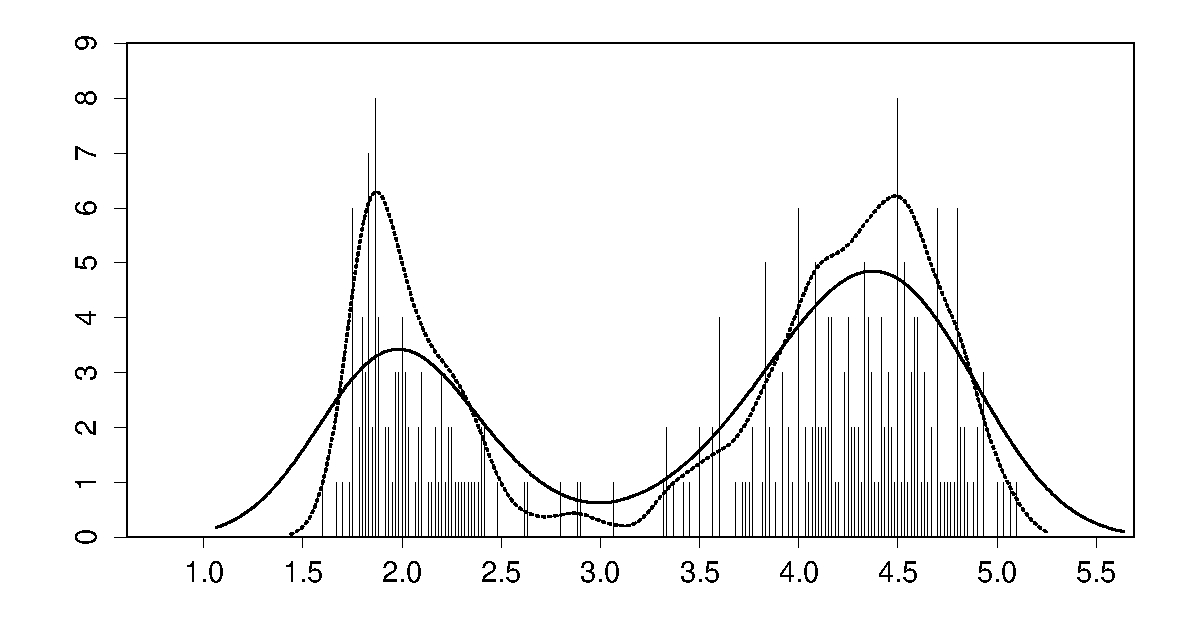
\includegraphics[width=.5\textwidth]{template-files/geys-2kern} %<< no file extension
  %%         --- .5\textwidth stands for 50% of text width
  \caption[Geyser data: binned histogram, Silverman's and another
    kernel]%<<-- Legend for the list of figures at the beginning of you thesis
  {Old Faithful Geyser eruption lengths, $n=272$; binned data and two
    (Gaussian) kernel density estimates ($\times 10$) with $h=h^*= .3348$
    and $h= .1$ (dotted).}% legend displayed below the graph.
  \label{fig:geys2}
\end{figure}

\section{To make a proof}
\begin{proof}
  $1 + 1 = 2$
\end{proof}

\section{To include \Rp code}
See information in Appendix~\ref{app:complement}.


\section{Other information}
Put a text between quotes: make sure to use nice quotes, such as `quote'.

Cite an article or book you refer shortly here, and then listed in the bibliography: \cite{ReferenceKey}.
%%--> in file   myReferences.bib  (same directory)
Or mention that \citeauthor{HamF85} (a person) or \citeauthor{StaWW91} (two
persons) have already done quite a bit work.

Referencing a different part of your work: please refer to Appendix~\ref{app:complement}.


%%% Local Variables: 
%%% mode: latex
%%% TeX-master: "MasterThesisSfS"
%%% End: 

%%\include{tex/Chapter...}
\ifdraft \else %XXX
  \chapter{Summary}
\label{s:Summary}

Summarize the presented work. Why is it useful to the research field or institute?


\section{Future Work}
\label{ss:FutureWork}

Possible ways to extend the work.


%%% Local Variables: 
%%% mode: latex
%%% TeX-master: "MasterThesisSfS"
%%% End: 

\fi %XXX
%%%%%%%%%%%%%%%%%%%%%%%%%%%%%%%%%%%%%%%%%%%%%%%%%
%%% Bibliography                              %%%
%%%%%%%%%%%%%%%%%%%%%%%%%%%%%%%%%%%%%%%%%%%%%%%%%
\addtocontents{toc}{\vspace{.5\baselineskip}}
\cleardoublepage
\phantomsection
\addcontentsline{toc}{chapter}{\protect\numberline{}{Bibliography}}
\bibliography{myReferences}
%% All books from our library (SfS) are already in a BiBTeX file
%% 'Assbib.bib' (included here as well), using
% \bibliography{myReferences,Assbib}
% ---------------------------------- instead of the above



%%%%%%%%%%%%%%%%%%%%%%%%%%%%%%%%%%%%%%%%%%%%%%%%% 
%%% Appendices (if needed, e.g. for R code)   %%%
%%%%%%%%%%%%%%%%%%%%%%%%%%%%%%%%%%%%%%%%%%%%%%%%%
\addtocontents{toc}{\vspace{.5\baselineskip}}
\appendix
\chapter{Further Material}

\section{Data and Methods}{
	\subsection{GDD}\label{app:gdd_examples}
		\cite{baileyUsingGrowingDegree2018} tabulates the corresponding GDD for each stage of wheat.
		\begin{table}[H]
			\centering
			\small
			\begin{tabular}{p{0.2\linewidth} p{0.57\linewidth}  p{0.13\linewidth}} 
				\toprule
				Stage  & Description    & GDD \\
				\hline Emergence & Leaf tip just emerging from above-ground coleoptyle. & $125-160$ \\
				\hline Leaf development & Two leaves unfolded. & $169-208$ \\
				\hline Tillering & First tiller visible  & $369-421$ \\
				\hline Stem elongation & First node detectable. & $592-659$ \\
				\hline Anthesis & Flowering commences; first anthers of cereals are visible. & $807-901$ \\
				\hline Seed fill & Seed fill begins. Caryopsis of cereals watery ripe (first grains have reached half of their final size). & $1068-1174$ \\
				\hline Dough stage & Soft dough stage, grain contents soft but dry, fingernail impression does not hold. & $1434-1556$ \\
				\hline Maturity complete & Grain is fully mature and drydown begins. Ready for harvest when dry. & $1538-1665$ \\
				\bottomrule
			\end{tabular}
		\end{table}
}


\section{Interpolation}
\begin{my_figure}[H]{width=1\textwidth}{interpol/2x3_loess_robust}
	\caption{The LOESS smoother \RobItPlot}
	\label{fig:interpol/2x3_loess_robust}
\end{my_figure}

\begin{my_figure}[H]{width=1\textwidth}{interpol/2x3_B-Splines_robust}
	\caption{B-splines \RobItPlot}
	\label{fig:interpol/2x3_B-Splines_robust}
\end{my_figure}

\begin{my_figure}[H]{width=1\textwidth}{interpol/2x3_DL_robust}
	\caption{A Double Logistic curve \RobItPlot}
	\label{fig:interpol/2x3_DL_robust}
\end{my_figure}

% \subsection{Skewness of LOOCV residuals}
% \begin{my_figure}[h]{width=0.6\textwidth}{interpol/res_cv}
% 	\caption{XXX caption XXX}
% 	\label{fig:interpol/res_cv}
% \end{my_figure}


\section{NDVI correction}
\todo[inline]{page breaks}

% step_plot/2017-201_ndvi.pdf 
% step_plot/2017-202_itpl.pdf 
% step_plot/2017-203_itpl_rew.pdf 
% step_plot/2017-204_ndvi_scl.pdf 
% step_plot/2017-205_show_res.pdf 
% step_plot/2017-206_corr.pdf 
% step_plot/2017-207_uncert.pdf 
% step_plot/2017-208_corr_itpl_rew.pdf

\begin{figure}[H]
	% \vspace{-15pt}
	% \centering
	% \begin{subfigure}[b]{0.42\textwidth}
	% 	\centering
	% 	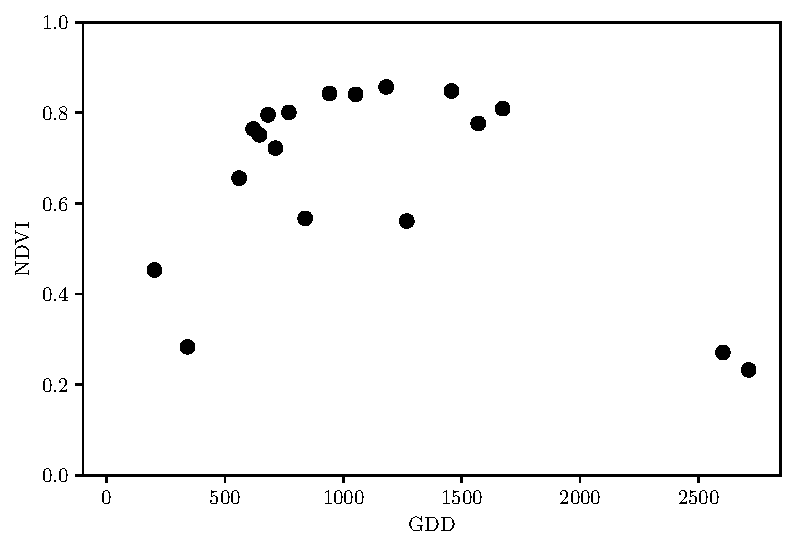
\includegraphics[width=\textwidth]{step_plot/2017-201_ndvi.pdf}
	% 	\vspace{-20pt}
	% 	\caption[NDVI {TS} with SCL45]%
	% 	{{\footnotesize NDVI {TS} with SCL45}}    
	% 	\label{fig:step_plot/2017-201_ndvi.pdf}
	% \end{subfigure}
	% \hfill
	
	\vskip\baselineskip
	\begin{subfigure}[b]{0.42\textwidth}  
		\centering 
		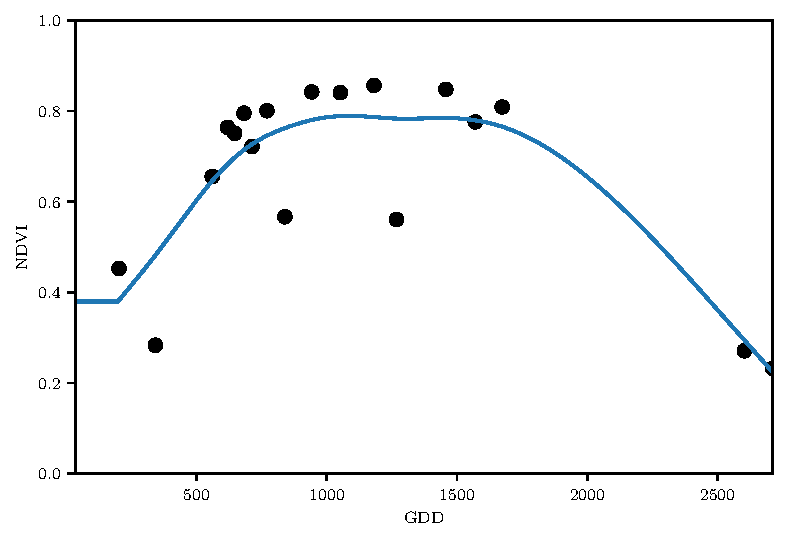
\includegraphics[width=\textwidth]{step_plot/2017-202_itpl.pdf}
		\vspace{-20pt}
		\caption[Interpolation via SS (only SCL45)]%
		{{\footnotesize Interpolation via SS (only SCL45)}}    
		\label{fig:step_plot/2017-202_itpl.pdf}
	\end{subfigure}
	% \begin{subfigure}[b]{0.42\textwidth}   
	% 	\centering 
	% 	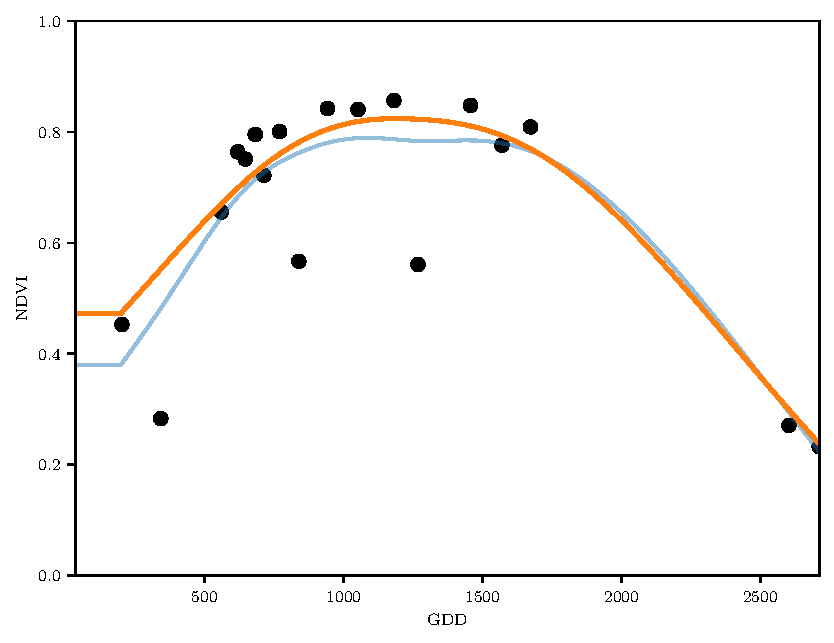
\includegraphics[width=\textwidth]{step_plot/2017-203_itpl_rew.pdf}
	% 	\vspace{-20pt}
	% 	\caption[Robustly reweighted fit]%
	% 	{{\footnotesize Robustly reweighted fit}}    
	% 	\label{fig:step_plot/2017-203_itpl_rew.pdf}
	% \end{subfigure}
	\hfill
	\begin{subfigure}[b]{0.42\textwidth}   
		\centering 
		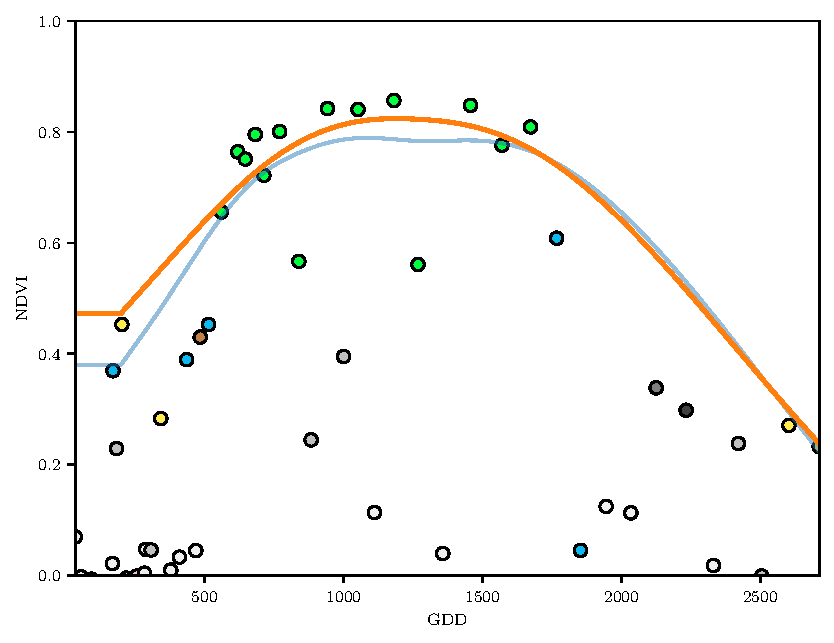
\includegraphics[width=\textwidth]{step_plot/2017-204_ndvi_scl.pdf}
		\vspace{-20pt}
		\caption[Now also consider other SCL-classes]%
		{\footnotesize Now also consider other SCL-classes}    
		\label{fig:step_plot/2017-204_ndvi_scl.pdf}
	\end{subfigure}

	\vskip\baselineskip
	\begin{subfigure}[b]{0.42\textwidth}   
		\centering 
		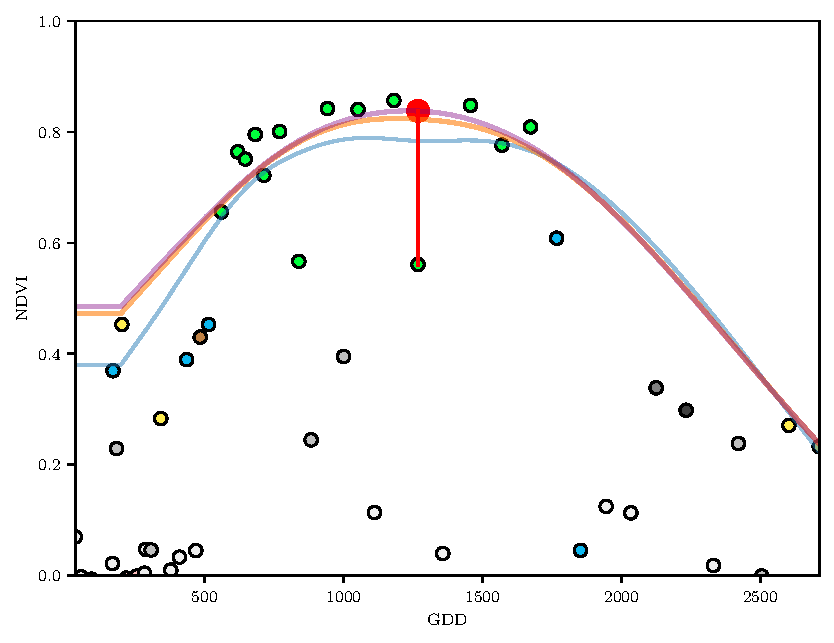
\includegraphics[width=\textwidth]{step_plot/2017-205_show_res.pdf}
		\vspace{-20pt}
		\caption[OOB estim. for each point using SCL45]%
		{{\footnotesize OOB estim. for each point using SCL45}}    
		\label{fig:step_plot/2017-205_show_res.pdf}
	\end{subfigure}
	\hfill
	\begin{subfigure}[b]{0.42\textwidth}   
		\centering 
		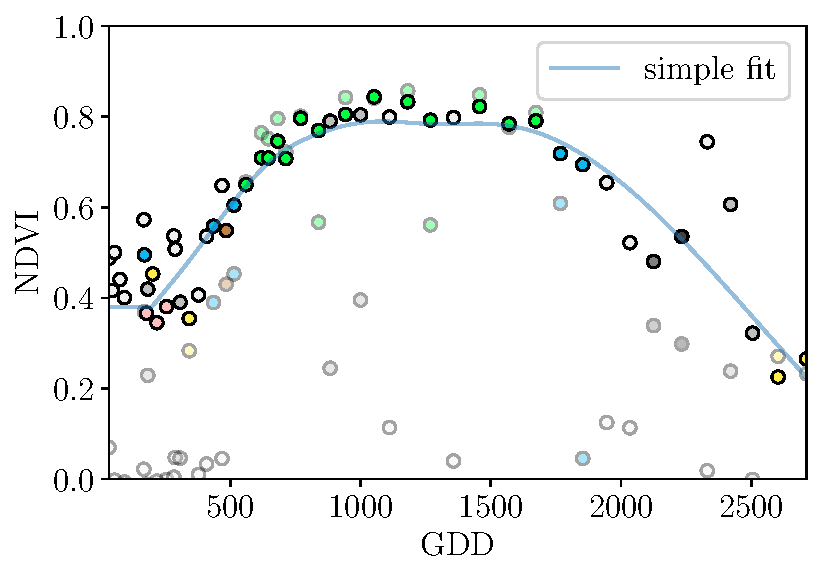
\includegraphics[width=\textwidth]{step_plot/2017-206_corr.pdf}
		\vspace{-20pt}
		\caption[Correct NDVI]%
		{\footnotesize Correct NDVI}    
		\label{fig:step_plot/2017-206_corr.pdf}
	\end{subfigure}

	\vskip\baselineskip
	\begin{subfigure}[b]{0.42\textwidth}   
		\centering 
		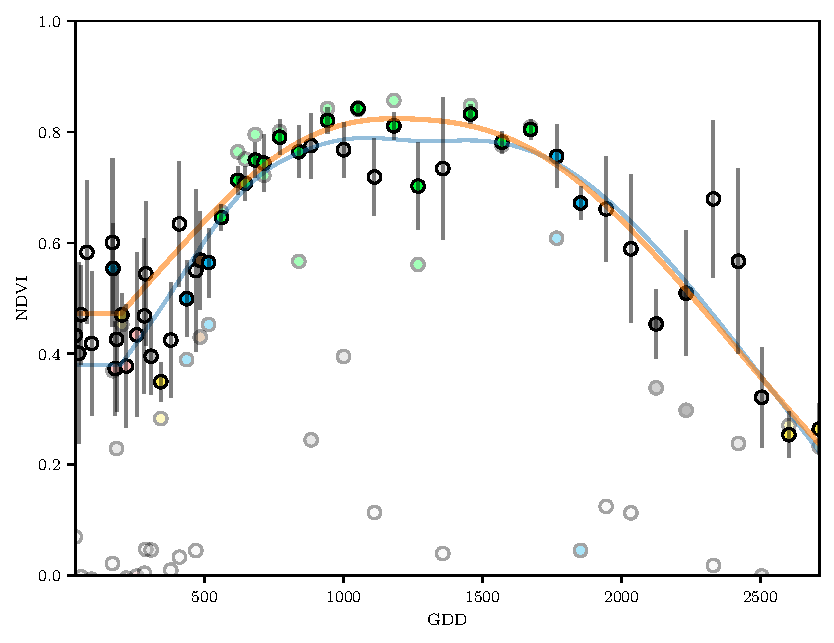
\includegraphics[width=\textwidth]{step_plot/2017-207_uncert.pdf}
		\vspace{-20pt}
		\caption[Estimate absolute errors]%
		{{\footnotesize Estimate absolute errors via statistical model}}    
		\label{fig:step_plot/2017-207_uncert.pdf}
	\end{subfigure}
	\hfill
	\begin{subfigure}[b]{0.42\textwidth}   
		\centering 
		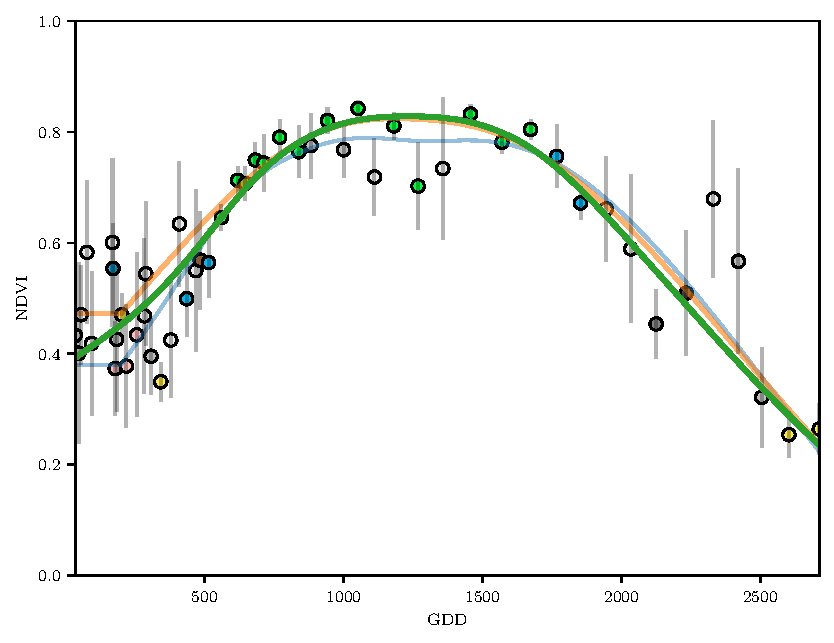
\includegraphics[width=\textwidth]{step_plot/2017-208_corr_itpl_rew.pdf}
		\vspace{-20pt}
		\caption[Interpolation (SS) on weights derived from uncertainties.]%
		{\footnotesize Robust interpolation on weights derived from uncertainties.}    
		\label{fig:step_plot/2017-208_corr_itpl_rew.pdf}
	\end{subfigure}
	\caption[Stepwise illustration of robust NDVI-Correction.]{Stepwise illustration of robust NDVI-Correction. For the color encoding of the SCL classes we refer to table~\ref{tab:satelite/scl_classes}.}
	\label{fig:step_plot_ndvi_corr}
\end{figure}


\begin{table}[H]
	\begin{center}
		\caption{Non-relative RMSE for yield prediction}.
		\small
		\begin{tabular}{lrrrrrrr}
\toprule
 & RF & OLS-SCL & OLS-all & MARS & GAM & LASSO & no-correction \\
\midrule
ss & {\cellcolor[HTML]{000000}} \color[HTML]{F1F1F1} 1.144 & {\cellcolor[HTML]{F1F1F1}} \color[HTML]{000000} 1.033 & {\cellcolor[HTML]{CACACA}} \color[HTML]{000000} 1.051 & {\cellcolor[HTML]{DDDDDD}} \color[HTML]{000000} 1.042 & {\cellcolor[HTML]{D4D4D4}} \color[HTML]{000000} 1.046 & {\cellcolor[HTML]{DDDDDD}} \color[HTML]{000000} 1.042 & {\cellcolor[HTML]{6A6A6A}} \color[HTML]{F1F1F1} 1.095 \\
dl & {\cellcolor[HTML]{222222}} \color[HTML]{F1F1F1} 1.150 & {\cellcolor[HTML]{ADADAD}} \color[HTML]{000000} 1.115 & {\cellcolor[HTML]{A7A7A7}} \color[HTML]{F1F1F1} 1.116 & {\cellcolor[HTML]{A7A7A7}} \color[HTML]{F1F1F1} 1.116 & {\cellcolor[HTML]{F1F1F1}} \color[HTML]{000000} 1.097 & {\cellcolor[HTML]{EDEDED}} \color[HTML]{000000} 1.098 & {\cellcolor[HTML]{000000}} \color[HTML]{F1F1F1} 1.159 \\
ss-rob & {\cellcolor[HTML]{000000}} \color[HTML]{F1F1F1} 1.144 & {\cellcolor[HTML]{F1F1F1}} \color[HTML]{000000} 1.054 & {\cellcolor[HTML]{A2A2A2}} \color[HTML]{F1F1F1} 1.084 & {\cellcolor[HTML]{878787}} \color[HTML]{F1F1F1} 1.094 & {\cellcolor[HTML]{C3C3C3}} \color[HTML]{000000} 1.072 & {\cellcolor[HTML]{C5C5C5}} \color[HTML]{000000} 1.071 & {\cellcolor[HTML]{8F8F8F}} \color[HTML]{F1F1F1} 1.091 \\
dl-rob & {\cellcolor[HTML]{000000}} \color[HTML]{F1F1F1} 1.159 & {\cellcolor[HTML]{4E4E4E}} \color[HTML]{F1F1F1} 1.128 & {\cellcolor[HTML]{696969}} \color[HTML]{F1F1F1} 1.117 & {\cellcolor[HTML]{F1F1F1}} \color[HTML]{000000} 1.064 & {\cellcolor[HTML]{A8A8A8}} \color[HTML]{F1F1F1} 1.093 & {\cellcolor[HTML]{888888}} \color[HTML]{F1F1F1} 1.105 & {\cellcolor[HTML]{060606}} \color[HTML]{F1F1F1} 1.156 \\
\bottomrule
\end{tabular}

		\label{tab:methods_vs_yieldprediction}
		\normalsize
	\end{center}
\end{table}


\begin{table}[H]
	\begin{center}
		\caption{Coefficient of determination (R\textsuperscript{2}) of yield prediction}
		\small
		\begin{tabular}{lrrrrrrr}
\toprule
 & RF & OLS-SCL & OLS-all & MARS & GAM & LASSO & no-correction \\
\midrule
ss & {\cellcolor[HTML]{F1F1F1}} \color[HTML]{000000} 0.431 & {\cellcolor[HTML]{000000}} \color[HTML]{F1F1F1} 0.486 & {\cellcolor[HTML]{272727}} \color[HTML]{F1F1F1} 0.477 & {\cellcolor[HTML]{141414}} \color[HTML]{F1F1F1} 0.481 & {\cellcolor[HTML]{1C1C1C}} \color[HTML]{F1F1F1} 0.479 & {\cellcolor[HTML]{141414}} \color[HTML]{F1F1F1} 0.481 & {\cellcolor[HTML]{878787}} \color[HTML]{F1F1F1} 0.455 \\
dl & {\cellcolor[HTML]{CFCFCF}} \color[HTML]{000000} 0.427 & {\cellcolor[HTML]{444444}} \color[HTML]{F1F1F1} 0.445 & {\cellcolor[HTML]{4A4A4A}} \color[HTML]{F1F1F1} 0.444 & {\cellcolor[HTML]{4A4A4A}} \color[HTML]{F1F1F1} 0.444 & {\cellcolor[HTML]{000000}} \color[HTML]{F1F1F1} 0.454 & {\cellcolor[HTML]{040404}} \color[HTML]{F1F1F1} 0.453 & {\cellcolor[HTML]{F1F1F1}} \color[HTML]{000000} 0.423 \\
ss-rob & {\cellcolor[HTML]{F1F1F1}} \color[HTML]{000000} 0.431 & {\cellcolor[HTML]{000000}} \color[HTML]{F1F1F1} 0.475 & {\cellcolor[HTML]{4E4E4E}} \color[HTML]{F1F1F1} 0.461 & {\cellcolor[HTML]{6A6A6A}} \color[HTML]{F1F1F1} 0.456 & {\cellcolor[HTML]{2D2D2D}} \color[HTML]{F1F1F1} 0.467 & {\cellcolor[HTML]{2B2B2B}} \color[HTML]{F1F1F1} 0.467 & {\cellcolor[HTML]{616161}} \color[HTML]{F1F1F1} 0.457 \\
dl-rob & {\cellcolor[HTML]{F1F1F1}} \color[HTML]{000000} 0.423 & {\cellcolor[HTML]{A2A2A2}} \color[HTML]{F1F1F1} 0.439 & {\cellcolor[HTML]{888888}} \color[HTML]{F1F1F1} 0.444 & {\cellcolor[HTML]{000000}} \color[HTML]{F1F1F1} 0.470 & {\cellcolor[HTML]{494949}} \color[HTML]{F1F1F1} 0.456 & {\cellcolor[HTML]{696969}} \color[HTML]{F1F1F1} 0.450 & {\cellcolor[HTML]{EBEBEB}} \color[HTML]{000000} 0.424 \\
\bottomrule
\end{tabular}

		\label{tab:methods_vs_yieldprediction_r2}
		\normalsize
	\end{center}
\end{table}

\subsection{OLS-SCL Model Outputs}\label{app:ols-scl-summary}
\lstinputlisting[title= R Summary of the NDVI correction model (cf. equation \refeq{eq:corr_lm})]{tex/chapters/misc/lm_scl.txt}
\lstinputlisting[title= R Summary of the NDVI correction model (cf. equation \refeq{eq:corr_lm_res})]{tex/chapters/misc/lm_scl_res.txt}


\todo[inline]{replace space before ref by tilda}
\todo[inline]{check quantile definitions}
\todo[inline]{schwarz weiss färbung der IS tabelle korrigieren}
\todo[inline]{so wenig wie möglich abkürzungen in den fig und table captions}
\todo[inline]{refer to data aviability}
\todo[inline]{abkürzungen Fourier und in tabellen}
\todo[inline]{figure spacing (caption zu nah dran --- manuell vspace einfügen wo nötig)}
\todo[inline]{italics für definitionen wie `variogramm' ja/nein --- einheitlich}
\todo[inline]{Gross schreiben von Fussnoten \& tabelleneinträgen + Satzzeichen}

% \chapter{Complementary information}
\label{app:complement}

Additional material. For example long mathematical derivations could be
given in the appendix. Or you could include part of your code that is
needed in printed form. You can add several Appendices to your thesis (as
you can include several chapters in the main part of your work).

\section{Including \Rp code with verbatim}
A simple (rather too simple, see~\ref{App:listings}) way to include code or
  {\it R} output is to use
\texttt{verbatim}. It just prints the text however it is (including all
spaces, ``strange'' symbols,...) in a slightly different font.
\begin{verbatim}
## loading packages
library(RBGL)
library(Rgraphviz)
library(boot)

## global variables
X_MAX <- 150

   This allows me to put as many s  p a   c es   as I want.
I can also use \ and ` and & and all the rest that is usually only 
accepted in the math mode.

I can also make as 
                  many 
             line 
    breaks as 
I want... and
             where I want. 
\end{verbatim}

But really recommended,  much better is the following:

\section{Including \Rp code with the \emph{listings} package}\label{App:listings}
However, it is much nicer to use the \emph{listings} package to include \Rp
code in your report. It allows you to number the lines, color the comments
differently than the code, and so on.
All the following is produced by simply writing
\verb! \lstinputlisting{figures/template-files/picture.R} !  in your \LaTeX\ ``code'':

\lstinputlisting{figures/template-files/picture.R}

or \verb!\lstinputlisting{/u/maechler/R/Pkgs/sfsmisc/R/misc/ellipse.R}! :

\lstinputlisting{misc/ellipse.R}% was /u/maechler/R/Pkgs/sfsmisc/R/misc/ellipse.R

\section{Using \texttt{Sweave} (or \texttt{knitr}) to include \Rp code (and more) in your report}
The easiest (and most elegant) way to include \Rp code and its output (and
have all your figures up to date with your report) is to use Sweave---or the
\href{https://cran.R-project.org/package=knitr}{\texttt{knitr}} R package with even more possibilities.
% You can find an introduction Sweave in \texttt{/u/sfs/StatSoftDoc/Sweave/Sweave-tutorial.pdf}.

Search the web to find lots of intro material on how to use Sweave or
\href{https://en.wikipedia.org/wiki/Knitr}{knitr (on Wikipedia)}.

%%% Local Variables: 
%%% mode: latex
%%% TeX-master: "MasterThesisSfS"
%%% End: 

% \chapter{Yet another appendix....}

\section{Description}
\begin{description}
\item[Something] details.
\item[Something else] other definition.
\end{description}

\section{Tables}
Refer to Table~\ref{tab:example} to see a left justified table with caption
on top.

\begin{table}[ht]
\centering
\caption[Test results]{\label{tab:example}Results.}
\begin{tabular}{ll}
\hline
\textbf{Student} & \textbf{Grade}\\
\hline
Marie  & $6$\\
Alain  & $5.5$\\
Josette  & $4.5$\\
Pierre  & $5$\\
\hline
\end{tabular}
\end{table}

%%% Local Variables: 
%%% mode: latex
%%% TeX-master: "MasterThesisSfS"
%%% End: 

% \chapter{2nd Appendix: More sophisticated R code listing} \label{appendix-more-R}

Chapter-wise listing of parts of R code, using
\begin{itemize}
\item \texttt{firstline=n1}
\item \texttt{lastline=n2}
\item \texttt{title=<text>}
\end{itemize}
e.g., for the first example below
\begin{verbatim}
\lstinputlisting[firstline=1,lastline=32,
                 title= \texttt{read\_irwls\_fn.R}]{../RCode/read_irwls_fn.R}
\end{verbatim}

% \section{Chapter 2} \label{app 2}

% \lstinputlisting[firstline=1,lastline=77,
% title=\texttt{analytic\_efficiency.R}]{../RCode/analytic_efficiency.R}
% %\lstinputlisting[firstline=,lastline=]{../RCode/???.R}

\bigskip% or even  \clearpage

%-----------------------------------------------------------------------------------------
\section{Chapter 5} \label{app 5}

% \lstinputlisting[firstline=1,lastline=71,
%                  title=\texttt{loss-fn\_rotated.R}]{../RCode/loss-fn_rotated.R}
\lstinputlisting[firstline=1,lastline=32,
                 title= \texttt{read\_irwls\_fn.R}]{misc/ellipse.R}

\medskip
                 
\lstinputlisting[firstline=1,lastline=45,
                 title=\texttt{plot.psi.R}]{misc/ellipse.R}
%\lstinputlisting[firstline=,lastline=]{../RCode/???.R}
%\lstinputlisting[firstline=,lastline=]{../RCode/???.R}

% \clearpage
%-----------------------------------------------------------------------------------------
% \section{Chapter 7} \label{app 7}

% \lstinputlisting[firstline=1,lastline=35,
%                  title= \texttt{stat.test} from \texttt{lmrob2-fn.R}]{../RCode/lmrob2-fn.R}
% \lstinputlisting[firstline=41,lastline=194,
%                  title=\texttt{M.optimal.ms} from \texttt{lmrob2-fn.R}]{../RCode/lmrob2-fn.R}
%\lstinputlisting[firstline=,lastline=]{../RCode/???.R}
%-----------------------------------------------------------------------------------------

%%% Local Variables:
%%% mode: latex
%%% TeX-master: "MasterThesisSfS"
%%% End:


\ifdraft \else %XXX
  %% Epilogue (optional)
  \addtocontents{toc}{\vspace{.5\baselineskip}}
  \cleardoublepage
  \phantomsection
  \addcontentsline{toc}{chapter}{\protect\numberline{}{Epilogue}}
  \markboth{Epilogue}{Epilogue}
  \chapter*{Epilogue}
\label{s:Epilogue}

A few final words.



%%% Local Variables: 
%%% mode: latex
%%% TeX-master: "MasterThesisSfS"
%%% End: 



  %%%%%%%%%%%%%%%%%%%%%%%%%%%%%%%%%%%%%%%%%%%%%%%%%% 
  %%% Declaration of originality (Do not remove!)%%%
  %%%%%%%%%%%%%%%%%%%%%%%%%%%%%%%%%%%%%%%%%%%%%%%%%%
  %% Instructions:
  %% -------------
  %% fill in the empty document confirmation-originality.pdf electronically
  %% print it out and sign it
  %% scan it in again and save the scan in this directory with name
  %% confirmation-originality-scan.pdf 
  %%
  %% General info on plagiarism:
  %% https://www.ethz.ch/students/en/studies/performance-assessments/plagiarism.html 
  \cleardoublepage
  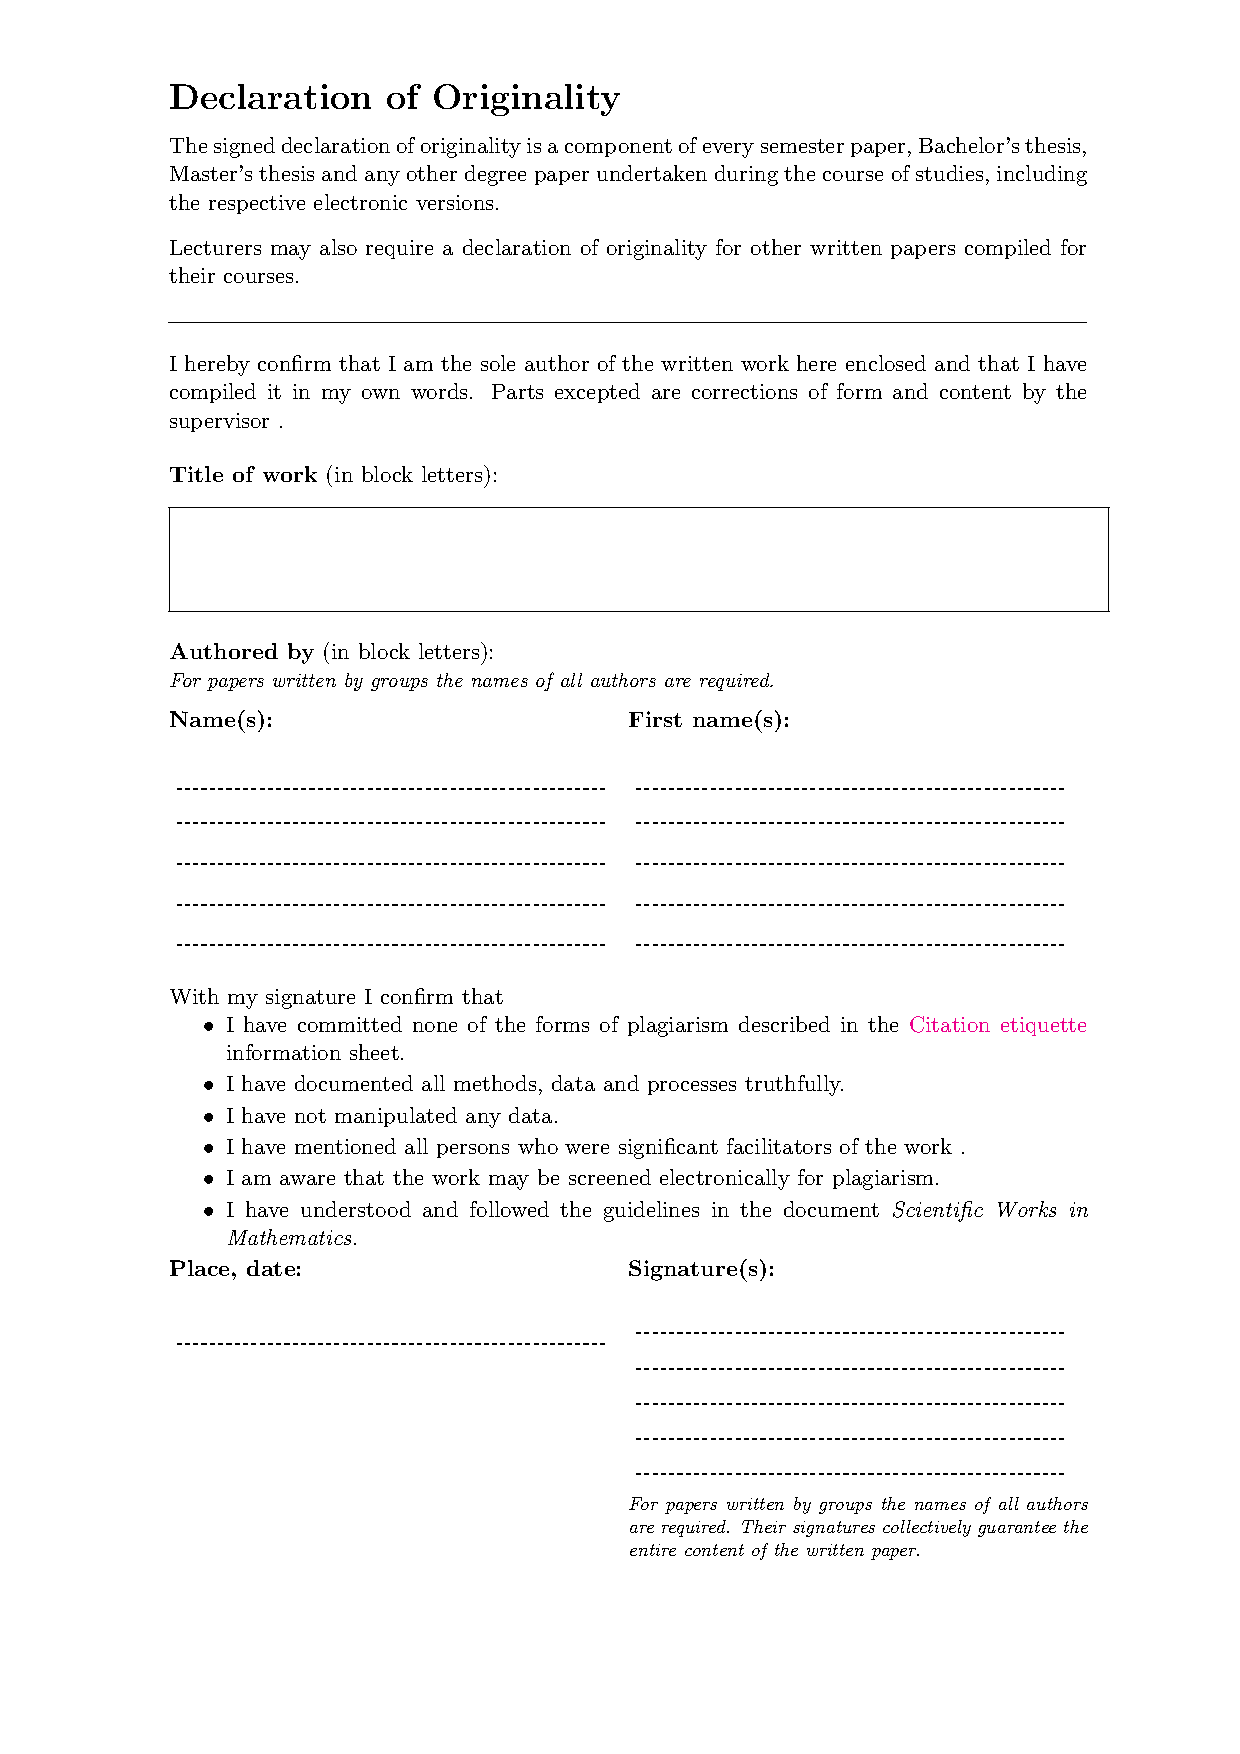
\includepdf[pages={-}, frame=true,scale=1]{misc/confirmation-originality.pdf}
\fi
\end{document}

%%% Local Variables:
%%% mode: latex
%%% TeX-master: "MasterThesisSfS"
%%% End:
